% Options for packages loaded elsewhere
\PassOptionsToPackage{unicode}{hyperref}
\PassOptionsToPackage{hyphens}{url}
%
\documentclass[
]{article}
\usepackage{amsmath,amssymb}
\usepackage{iftex}
\ifPDFTeX
  \usepackage[T1]{fontenc}
  \usepackage[utf8]{inputenc}
  \usepackage{textcomp} % provide euro and other symbols
\else % if luatex or xetex
  \usepackage{unicode-math} % this also loads fontspec
  \defaultfontfeatures{Scale=MatchLowercase}
  \defaultfontfeatures[\rmfamily]{Ligatures=TeX,Scale=1}
\fi
\usepackage{lmodern}
\ifPDFTeX\else
  % xetex/luatex font selection
\fi
% Use upquote if available, for straight quotes in verbatim environments
\IfFileExists{upquote.sty}{\usepackage{upquote}}{}
\IfFileExists{microtype.sty}{% use microtype if available
  \usepackage[]{microtype}
  \UseMicrotypeSet[protrusion]{basicmath} % disable protrusion for tt fonts
}{}
\makeatletter
\@ifundefined{KOMAClassName}{% if non-KOMA class
  \IfFileExists{parskip.sty}{%
    \usepackage{parskip}
  }{% else
    \setlength{\parindent}{0pt}
    \setlength{\parskip}{6pt plus 2pt minus 1pt}}
}{% if KOMA class
  \KOMAoptions{parskip=half}}
\makeatother
\usepackage{xcolor}
\usepackage[margin=1in]{geometry}
\usepackage{color}
\usepackage{fancyvrb}
\newcommand{\VerbBar}{|}
\newcommand{\VERB}{\Verb[commandchars=\\\{\}]}
\DefineVerbatimEnvironment{Highlighting}{Verbatim}{commandchars=\\\{\}}
% Add ',fontsize=\small' for more characters per line
\usepackage{framed}
\definecolor{shadecolor}{RGB}{248,248,248}
\newenvironment{Shaded}{\begin{snugshade}}{\end{snugshade}}
\newcommand{\AlertTok}[1]{\textcolor[rgb]{0.94,0.16,0.16}{#1}}
\newcommand{\AnnotationTok}[1]{\textcolor[rgb]{0.56,0.35,0.01}{\textbf{\textit{#1}}}}
\newcommand{\AttributeTok}[1]{\textcolor[rgb]{0.13,0.29,0.53}{#1}}
\newcommand{\BaseNTok}[1]{\textcolor[rgb]{0.00,0.00,0.81}{#1}}
\newcommand{\BuiltInTok}[1]{#1}
\newcommand{\CharTok}[1]{\textcolor[rgb]{0.31,0.60,0.02}{#1}}
\newcommand{\CommentTok}[1]{\textcolor[rgb]{0.56,0.35,0.01}{\textit{#1}}}
\newcommand{\CommentVarTok}[1]{\textcolor[rgb]{0.56,0.35,0.01}{\textbf{\textit{#1}}}}
\newcommand{\ConstantTok}[1]{\textcolor[rgb]{0.56,0.35,0.01}{#1}}
\newcommand{\ControlFlowTok}[1]{\textcolor[rgb]{0.13,0.29,0.53}{\textbf{#1}}}
\newcommand{\DataTypeTok}[1]{\textcolor[rgb]{0.13,0.29,0.53}{#1}}
\newcommand{\DecValTok}[1]{\textcolor[rgb]{0.00,0.00,0.81}{#1}}
\newcommand{\DocumentationTok}[1]{\textcolor[rgb]{0.56,0.35,0.01}{\textbf{\textit{#1}}}}
\newcommand{\ErrorTok}[1]{\textcolor[rgb]{0.64,0.00,0.00}{\textbf{#1}}}
\newcommand{\ExtensionTok}[1]{#1}
\newcommand{\FloatTok}[1]{\textcolor[rgb]{0.00,0.00,0.81}{#1}}
\newcommand{\FunctionTok}[1]{\textcolor[rgb]{0.13,0.29,0.53}{\textbf{#1}}}
\newcommand{\ImportTok}[1]{#1}
\newcommand{\InformationTok}[1]{\textcolor[rgb]{0.56,0.35,0.01}{\textbf{\textit{#1}}}}
\newcommand{\KeywordTok}[1]{\textcolor[rgb]{0.13,0.29,0.53}{\textbf{#1}}}
\newcommand{\NormalTok}[1]{#1}
\newcommand{\OperatorTok}[1]{\textcolor[rgb]{0.81,0.36,0.00}{\textbf{#1}}}
\newcommand{\OtherTok}[1]{\textcolor[rgb]{0.56,0.35,0.01}{#1}}
\newcommand{\PreprocessorTok}[1]{\textcolor[rgb]{0.56,0.35,0.01}{\textit{#1}}}
\newcommand{\RegionMarkerTok}[1]{#1}
\newcommand{\SpecialCharTok}[1]{\textcolor[rgb]{0.81,0.36,0.00}{\textbf{#1}}}
\newcommand{\SpecialStringTok}[1]{\textcolor[rgb]{0.31,0.60,0.02}{#1}}
\newcommand{\StringTok}[1]{\textcolor[rgb]{0.31,0.60,0.02}{#1}}
\newcommand{\VariableTok}[1]{\textcolor[rgb]{0.00,0.00,0.00}{#1}}
\newcommand{\VerbatimStringTok}[1]{\textcolor[rgb]{0.31,0.60,0.02}{#1}}
\newcommand{\WarningTok}[1]{\textcolor[rgb]{0.56,0.35,0.01}{\textbf{\textit{#1}}}}
\usepackage{graphicx}
\makeatletter
\def\maxwidth{\ifdim\Gin@nat@width>\linewidth\linewidth\else\Gin@nat@width\fi}
\def\maxheight{\ifdim\Gin@nat@height>\textheight\textheight\else\Gin@nat@height\fi}
\makeatother
% Scale images if necessary, so that they will not overflow the page
% margins by default, and it is still possible to overwrite the defaults
% using explicit options in \includegraphics[width, height, ...]{}
\setkeys{Gin}{width=\maxwidth,height=\maxheight,keepaspectratio}
% Set default figure placement to htbp
\makeatletter
\def\fps@figure{htbp}
\makeatother
\setlength{\emergencystretch}{3em} % prevent overfull lines
\providecommand{\tightlist}{%
  \setlength{\itemsep}{0pt}\setlength{\parskip}{0pt}}
\setcounter{secnumdepth}{-\maxdimen} % remove section numbering
\usepackage{booktabs}
\usepackage{longtable}
\usepackage{array}
\usepackage{multirow}
\usepackage{wrapfig}
\usepackage{float}
\usepackage{colortbl}
\usepackage{pdflscape}
\usepackage{tabu}
\usepackage{threeparttable}
\usepackage{threeparttablex}
\usepackage[normalem]{ulem}
\usepackage{makecell}
\usepackage{xcolor}
\ifLuaTeX
  \usepackage{selnolig}  % disable illegal ligatures
\fi
\usepackage{bookmark}
\IfFileExists{xurl.sty}{\usepackage{xurl}}{} % add URL line breaks if available
\urlstyle{same}
\hypersetup{
  pdftitle={Task 1: Wage Prediction Model: Data Exploration, Model Selection, and Prediction},
  pdfauthor={Fabio Burri, Mischa Haenen, Robin Galeazzi, and Timon Galeazzi},
  hidelinks,
  pdfcreator={LaTeX via pandoc}}

\title{Task 1: Wage Prediction Model: Data Exploration, Model Selection,
and Prediction}
\author{Fabio Burri, Mischa Haenen, Robin Galeazzi, and Timon Galeazzi}
\date{2024-05-27}

\begin{document}
\maketitle

\subsection{Data Exploration and Preparation: Analyze the features in
your dataset to select relevant predictors for the
wage.}\label{data-exploration-and-preparation-analyze-the-features-in-your-dataset-to-select-relevant-predictors-for-the-wage.}

\begin{Shaded}
\begin{Highlighting}[]
\CommentTok{\# Load the dataset}
\CommentTok{\# getwd()}
\CommentTok{\# setwd("./3.Applied{-}Supervised{-}Learning{-}Groupwork")}
\FunctionTok{load}\NormalTok{(}\StringTok{"./data\_wage.RData"}\NormalTok{)}

\CommentTok{\# Handle missing values by removing rows with NAs}
\NormalTok{data\_wage }\OtherTok{\textless{}{-}} \FunctionTok{na.omit}\NormalTok{(data)}
\end{Highlighting}
\end{Shaded}

Then our idea was to get a quick overview of the dataset. Which
dimensions does the dataset have? Which variable types are used?

\begin{Shaded}
\begin{Highlighting}[]
\CommentTok{\# Display dataset dimensions and basic structure}
\FunctionTok{dim}\NormalTok{(data\_wage)}
\end{Highlighting}
\end{Shaded}

\begin{verbatim}
## [1] 10809    78
\end{verbatim}

\begin{Shaded}
\begin{Highlighting}[]
\FunctionTok{summary}\NormalTok{(data\_wage)}
\end{Highlighting}
\end{Shaded}

\begin{verbatim}
##                      gender          age                           country    
##  Female                 :1571   25-29  :3008   United States of America:2505  
##  Male                   :9135   30-34  :2064   India                   :1576  
##  Prefer not to say      :  72   22-24  :1914   China                   : 563  
##  Prefer to self-describe:  31   35-39  :1195   Other                   : 468  
##                                 18-21  : 838   Brazil                  : 412  
##                                 40-44  : 717   Russia                  : 380  
##                                 (Other):1073   (Other)                 :4905  
##                                                              education   
##  Bachelor’s degree                                                :2990  
##  Doctoral degree                                                  :1869  
##  I prefer not to answer                                           :  74  
##  Master’s degree                                                  :5209  
##  Professional degree                                              : 281  
##  Some college/university study without earning a bachelor’s degree: 386  
##                                                                          
##                                                    undergraduate_major
##  Computer science (software engineering, etc.)               :4239    
##  Engineering (non-computer focused)                          :1704    
##  Mathematics or statistics                                   :1545    
##  A business discipline (accounting, economics, finance, etc.): 884    
##  Physics or astronomy                                        : 626    
##  Information technology, networking, or system administration: 447    
##  (Other)                                                     :1364    
##                job_role                                      industry   
##  Data Scientist    :2505   Computers/Technology                  :3032  
##  Software Engineer :1800   I am a student                        :1361  
##  Student           :1588   Academics/Education                   :1317  
##  Data Analyst      :1022   Accounting/Finance                    : 878  
##  Research Scientist: 662   Online Service/Internet-based Services: 541  
##  Other             : 606   Other                                 : 498  
##  (Other)           :2626   (Other)                               :3182  
##  years_experience
##  0-1    :2604    
##  1-2    :1974    
##  5-11   :1421    
##  2-3    :1381    
##  3-4    : 953    
##  4-5    : 854    
##  (Other):1622    
##                                                                                      ML_atwork   
##  I do not know                                                                            : 815  
##  No (we do not use ML methods)                                                            :2171  
##  We are exploring ML methods (and may one day put a model into production)                :2529  
##  We have well established ML methods (i.e., models in production for more than 2 years)   :1756  
##  We recently started using ML methods (i.e., models in production for less than 2 years)  :2299  
##  We use ML methods for generating insights (but do not put working models into production):1239  
##                                                                                                  
##  Activities_Analyze.and.understand.data.to.influence.product.or.business.decisions
##  Min.   :0.000                                                                    
##  1st Qu.:0.000                                                                    
##  Median :1.000                                                                    
##  Mean   :0.541                                                                    
##  3rd Qu.:1.000                                                                    
##  Max.   :1.000                                                                    
##                                                                                   
##  Activities_Build.and.or.run.a.machine.learning.service.that.operationally.improves.my.product.or.workflows
##  Min.   :0.0000                                                                                            
##  1st Qu.:0.0000                                                                                            
##  Median :0.0000                                                                                            
##  Mean   :0.3128                                                                                            
##  3rd Qu.:1.0000                                                                                            
##  Max.   :1.0000                                                                                            
##                                                                                                            
##  Activities_Build.and.or.run.the.data.infrastructure.that.my.business.uses.for.storing..analyzing..and.operationalizing.data
##  Min.   :0.0000                                                                                                             
##  1st Qu.:0.0000                                                                                                             
##  Median :0.0000                                                                                                             
##  Mean   :0.3126                                                                                                             
##  3rd Qu.:1.0000                                                                                                             
##  Max.   :1.0000                                                                                                             
##                                                                                                                             
##  Activities_Build.prototypes.to.explore.applying.machine.learning.to.new.areas
##  Min.   :0.0000                                                               
##  1st Qu.:0.0000                                                               
##  Median :0.0000                                                               
##  Mean   :0.4266                                                               
##  3rd Qu.:1.0000                                                               
##  Max.   :1.0000                                                               
##                                                                               
##  Activities_Do.research.that.advances.the.state.of.the.art.of.machine.learning
##  Min.   :0.000                                                                
##  1st Qu.:0.000                                                                
##  Median :0.000                                                                
##  Mean   :0.259                                                                
##  3rd Qu.:1.000                                                                
##  Max.   :1.000                                                                
##                                                                               
##  Activities_None.of.these.activities.are.an.important.part.of.my.role.at.work
##  Min.   :0.000                                                               
##  1st Qu.:0.000                                                               
##  Median :0.000                                                               
##  Mean   :0.154                                                               
##  3rd Qu.:0.000                                                               
##  Max.   :1.000                                                               
##                                                                              
##  Notebooks_Kaggle.Kernels Notebooks_Google.Colab Notebooks_Azure.Notebook
##  Min.   :0.0000           Min.   :0.0000         Min.   :0.0000          
##  1st Qu.:0.0000           1st Qu.:0.0000         1st Qu.:0.0000          
##  Median :0.0000           Median :0.0000         Median :0.0000          
##  Mean   :0.3335           Mean   :0.1944         Mean   :0.0741          
##  3rd Qu.:1.0000           3rd Qu.:0.0000         3rd Qu.:0.0000          
##  Max.   :1.0000           Max.   :1.0000         Max.   :1.0000          
##                                                                          
##  Notebooks_Google.Cloud.Datalab Notebooks_JupyterHub.Binder Notebooks_None  
##  Min.   :0.00000                Min.   :0.0000              Min.   :0.0000  
##  1st Qu.:0.00000                1st Qu.:0.0000              1st Qu.:0.0000  
##  Median :0.00000                Median :0.0000              Median :0.0000  
##  Mean   :0.07327                Mean   :0.2774              Mean   :0.3796  
##  3rd Qu.:0.00000                3rd Qu.:1.0000              3rd Qu.:1.0000  
##  Max.   :1.00000                Max.   :1.0000              Max.   :1.0000  
##                                                                             
##  cloud_Google.Cloud.Platform..GCP. cloud_Amazon.Web.Services..AWS.
##  Min.   :0.0000                    Min.   :0.0000                 
##  1st Qu.:0.0000                    1st Qu.:0.0000                 
##  Median :0.0000                    Median :0.0000                 
##  Mean   :0.2756                    Mean   :0.4596                 
##  3rd Qu.:1.0000                    3rd Qu.:1.0000                 
##  Max.   :1.0000                    Max.   :1.0000                 
##                                                                   
##  cloud_Microsoft.Azure cloud_IBM.Cloud   cloud_Alibaba.Cloud
##  Min.   :0.0000        Min.   :0.00000   Min.   :0.00000    
##  1st Qu.:0.0000        1st Qu.:0.00000   1st Qu.:0.00000    
##  Median :0.0000        Median :0.00000   Median :0.00000    
##  Mean   :0.2329        Mean   :0.06874   Mean   :0.02692    
##  3rd Qu.:0.0000        3rd Qu.:0.00000   3rd Qu.:0.00000    
##  Max.   :1.0000        Max.   :1.00000   Max.   :1.00000    
##                                                             
##  cloud_I.have.not.used.any.cloud.providers Programming_Python Programming_R   
##  Min.   :0.0000                            Min.   :0.0000     Min.   :0.0000  
##  1st Qu.:0.0000                            1st Qu.:1.0000     1st Qu.:0.0000  
##  Median :0.0000                            Median :1.0000     Median :0.0000  
##  Mean   :0.3209                            Mean   :0.8832     Mean   :0.4208  
##  3rd Qu.:1.0000                            3rd Qu.:1.0000     3rd Qu.:1.0000  
##  Max.   :1.0000                            Max.   :1.0000     Max.   :1.0000  
##                                                                               
##  Programming_SQL  Programming_Bash Programming_Java
##  Min.   :0.0000   Min.   :0.0000   Min.   :0.0000  
##  1st Qu.:0.0000   1st Qu.:0.0000   1st Qu.:0.0000  
##  Median :1.0000   Median :0.0000   Median :0.0000  
##  Mean   :0.5478   Mean   :0.1929   Mean   :0.2363  
##  3rd Qu.:1.0000   3rd Qu.:0.0000   3rd Qu.:0.0000  
##  Max.   :1.0000   Max.   :1.0000   Max.   :1.0000  
##                                                    
##  Programming_Javascript.Typescript Programming_Visual.Basic.VBA
##  Min.   :0.000                     Min.   :0.0000              
##  1st Qu.:0.000                     1st Qu.:0.0000              
##  Median :0.000                     Median :0.0000              
##  Mean   :0.212                     Mean   :0.0841              
##  3rd Qu.:0.000                     3rd Qu.:0.0000              
##  Max.   :1.000                     Max.   :1.0000              
##                                                                
##  Programming_C.C.. Programming_MATLAB Programming_Scala Programming_Julia
##  Min.   :0.0000    Min.   :0.0000     Min.   :0.00000   Min.   :0.00000  
##  1st Qu.:0.0000    1st Qu.:0.0000     1st Qu.:0.00000   1st Qu.:0.00000  
##  Median :0.0000    Median :0.0000     Median :0.00000   Median :0.00000  
##  Mean   :0.2496    Mean   :0.1548     Mean   :0.05791   Mean   :0.01508  
##  3rd Qu.:0.0000    3rd Qu.:0.0000     3rd Qu.:0.00000   3rd Qu.:0.00000  
##  Max.   :1.0000    Max.   :1.0000     Max.   :1.00000   Max.   :1.00000  
##                                                                          
##  Programming_SAS.STATA Programming_language_used_most_often
##  Min.   :0.00000       Python :5754                        
##  1st Qu.:0.00000       R      :1500                        
##  Median :0.00000       SQL    : 973                        
##  Mean   :0.06994       Java   : 598                        
##  3rd Qu.:0.00000       C/C++  : 447                        
##  Max.   :1.00000       C#/.NET: 309                        
##                        (Other):1228                        
##  ML_framework_Scikit.Learn ML_framework_TensorFlow ML_framework_Keras
##  Min.   :0.000             Min.   :0.0000          Min.   :0.0000    
##  1st Qu.:0.000             1st Qu.:0.0000          1st Qu.:0.0000    
##  Median :1.000             Median :1.0000          Median :0.0000    
##  Mean   :0.702             Mean   :0.5701          Mean   :0.4681    
##  3rd Qu.:1.000             3rd Qu.:1.0000          3rd Qu.:1.0000    
##  Max.   :1.000             Max.   :1.0000          Max.   :1.0000    
##                                                                      
##  ML_framework_PyTorch ML_framework_Spark.MLlib ML_framework_H20 
##  Min.   :0.0000       Min.   :0.0000           Min.   :0.00000  
##  1st Qu.:0.0000       1st Qu.:0.0000           1st Qu.:0.00000  
##  Median :0.0000       Median :0.0000           Median :0.00000  
##  Mean   :0.2163       Mean   :0.1384           Mean   :0.08844  
##  3rd Qu.:0.0000       3rd Qu.:0.0000           3rd Qu.:0.00000  
##  Max.   :1.0000       Max.   :1.0000           Max.   :1.00000  
##                                                                 
##  ML_framework_Caret ML_framework_Xgboost ML_framework_randomForest
##  Min.   :0.0000     Min.   :0.0000       Min.   :0.0000           
##  1st Qu.:0.0000     1st Qu.:0.0000       1st Qu.:0.0000           
##  Median :0.0000     Median :0.0000       Median :0.0000           
##  Mean   :0.1453     Mean   :0.3318       Mean   :0.3482           
##  3rd Qu.:0.0000     3rd Qu.:1.0000       3rd Qu.:1.0000           
##  Max.   :1.0000     Max.   :1.0000       Max.   :1.0000           
##                                                                   
##  ML_framework_None Visualization_ggplot2 Visualization_Matplotlib
##  Min.   :0.000     Min.   :0.0000        Min.   :0.0000          
##  1st Qu.:0.000     1st Qu.:0.0000        1st Qu.:0.0000          
##  Median :0.000     Median :0.0000        Median :1.0000          
##  Mean   :0.118     Mean   :0.4739        Mean   :0.7495          
##  3rd Qu.:0.000     3rd Qu.:1.0000        3rd Qu.:1.0000          
##  Max.   :1.000     Max.   :1.0000        Max.   :1.0000          
##                                                                  
##  Visualization_Altair Visualization_Shiny Visualization_Plotly
##  Min.   :0.00000      Min.   :0.0000      Min.   :0.0000      
##  1st Qu.:0.00000      1st Qu.:0.0000      1st Qu.:0.0000      
##  Median :0.00000      Median :0.0000      Median :0.0000      
##  Mean   :0.01397      Mean   :0.1777      Mean   :0.3432      
##  3rd Qu.:0.00000      3rd Qu.:0.0000      3rd Qu.:1.0000      
##  Max.   :1.00000      Max.   :1.0000      Max.   :1.0000      
##                                                               
##  Visualization_None          percent_actively.coding
##  Min.   :0.00000    0% of my time        : 103      
##  1st Qu.:0.00000    1% to 25% of my time :2155      
##  Median :0.00000    100% of my time      : 276      
##  Mean   :0.07429    25% to 49% of my time:2969      
##  3rd Qu.:0.00000    50% to 74% of my time:3458      
##  Max.   :1.00000    75% to 99% of my time:1848      
##                                                     
##                     How.long.have.you.been.writing.code.to.analyze.data.
##  1-2 years                                    :3030                     
##  3-5 years                                    :2700                     
##  < 1 year                                     :2147                     
##  5-10 years                                   :1548                     
##  10-20 years                                  : 810                     
##  I have never written code but I want to learn: 261                     
##  (Other)                                      : 313                     
##                              For.how.many.years.have.you.used.machine.learning.methods..at.work.or.in.school..
##  < 1 year                                                             :3306                                   
##  1-2 years                                                            :2960                                   
##  2-3 years                                                            :1411                                   
##  3-4 years                                                            : 782                                   
##  I have never studied machine learning but plan to learn in the future: 770                                   
##  5-10 years                                                           : 650                                   
##  (Other)                                                              : 930                                   
##  Do.you.consider.yourself.to.be.a.data.scientist. data_Categorical.Data
##  Definitely not: 813                              Min.   :0.0000       
##  Definitely yes:2964                              1st Qu.:0.0000       
##  Maybe         :2315                              Median :0.0000       
##  Probably not  :1728                              Mean   :0.4823       
##  Probably yes  :2989                              3rd Qu.:1.0000       
##                                                   Max.   :1.0000       
##                                                                        
##  data_Genetic.Data data_Geospatial.Data data_Image.Data  data_Numerical.Data
##  Min.   :0.00000   Min.   :0.0000       Min.   :0.0000   Min.   :0.0000     
##  1st Qu.:0.00000   1st Qu.:0.0000       1st Qu.:0.0000   1st Qu.:0.0000     
##  Median :0.00000   Median :0.0000       Median :0.0000   Median :1.0000     
##  Mean   :0.06088   Mean   :0.1416       Mean   :0.2884   Mean   :0.6337     
##  3rd Qu.:0.00000   3rd Qu.:0.0000       3rd Qu.:1.0000   3rd Qu.:1.0000     
##  Max.   :1.00000   Max.   :1.0000       Max.   :1.0000   Max.   :1.0000     
##                                                                             
##  data_Sensor.Data data_Tabular.Data data_text.Data   data_Time.Series.Data
##  Min.   :0.0000   Min.   :0.0000    Min.   :0.0000   Min.   :0.0000       
##  1st Qu.:0.0000   1st Qu.:0.0000    1st Qu.:0.0000   1st Qu.:0.0000       
##  Median :0.0000   Median :0.0000    Median :1.0000   Median :0.0000       
##  Mean   :0.1528   Mean   :0.4421    Mean   :0.5022   Mean   :0.4699       
##  3rd Qu.:0.0000   3rd Qu.:1.0000    3rd Qu.:1.0000   3rd Qu.:1.0000       
##  Max.   :1.0000   Max.   :1.0000    Max.   :1.0000   Max.   :1.0000       
##                                                                           
##  data_Video.Data  explainability.model_Examine.individual.model.coefficients
##  Min.   :0.0000   Min.   :0.0000                                            
##  1st Qu.:0.0000   1st Qu.:0.0000                                            
##  Median :0.0000   Median :0.0000                                            
##  Mean   :0.0779   Mean   :0.2268                                            
##  3rd Qu.:0.0000   3rd Qu.:0.0000                                            
##  Max.   :1.0000   Max.   :1.0000                                            
##                                                                             
##  explainability.model_examine.feature.correlations
##  Min.   :0.0000                                   
##  1st Qu.:0.0000                                   
##  Median :0.0000                                   
##  Mean   :0.3369                                   
##  3rd Qu.:1.0000                                   
##  Max.   :1.0000                                   
##                                                   
##  explainability.model_Examine.feature.importances
##  Min.   :0.000                                   
##  1st Qu.:0.000                                   
##  Median :0.000                                   
##  Mean   :0.372                                   
##  3rd Qu.:1.000                                   
##  Max.   :1.000                                   
##                                                  
##  explainability.model_Create.partial.dependence.plots
##  Min.   :0.0000                                      
##  1st Qu.:0.0000                                      
##  Median :0.0000                                      
##  Mean   :0.1192                                      
##  3rd Qu.:0.0000                                      
##  Max.   :1.0000                                      
##                                                      
##  explainability.model_LIME.functions explainability.model_SHAP.functions
##  Min.   :0.00000                     Min.   :0.00000                    
##  1st Qu.:0.00000                     1st Qu.:0.00000                    
##  Median :0.00000                     Median :0.00000                    
##  Mean   :0.05995                     Mean   :0.04663                    
##  3rd Qu.:0.00000                     3rd Qu.:0.00000                    
##  Max.   :1.00000                     Max.   :1.00000                    
##                                                                         
##  explainability.model_None.I.do.not.use.these.model.explanation.techniques
##  Min.   :0.000                                                            
##  1st Qu.:0.000                                                            
##  Median :0.000                                                            
##  Mean   :0.101                                                            
##  3rd Qu.:0.000                                                            
##  Max.   :1.000                                                            
##                                                                           
##       wage       
##  Min.   :     0  
##  1st Qu.:  6811  
##  Median : 34780  
##  Mean   : 53048  
##  3rd Qu.: 75687  
##  Max.   :551774  
## 
\end{verbatim}

\begin{Shaded}
\begin{Highlighting}[]
\FunctionTok{head}\NormalTok{(data\_wage, }\DecValTok{1}\NormalTok{)}
\end{Highlighting}
\end{Shaded}

\begin{verbatim}
##   gender   age                  country       education
## 3 Female 30-34 United States of America Master’s degree
##                             undergraduate_major       job_role       industry
## 3 Computer science (software engineering, etc.) Data Scientist I am a student
##   years_experience     ML_atwork
## 3              0-1 I do not know
##   Activities_Analyze.and.understand.data.to.influence.product.or.business.decisions
## 3                                                                                 1
##   Activities_Build.and.or.run.a.machine.learning.service.that.operationally.improves.my.product.or.workflows
## 3                                                                                                          0
##   Activities_Build.and.or.run.the.data.infrastructure.that.my.business.uses.for.storing..analyzing..and.operationalizing.data
## 3                                                                                                                           0
##   Activities_Build.prototypes.to.explore.applying.machine.learning.to.new.areas
## 3                                                                             0
##   Activities_Do.research.that.advances.the.state.of.the.art.of.machine.learning
## 3                                                                             0
##   Activities_None.of.these.activities.are.an.important.part.of.my.role.at.work
## 3                                                                            0
##   Notebooks_Kaggle.Kernels Notebooks_Google.Colab Notebooks_Azure.Notebook
## 3                        0                      0                        0
##   Notebooks_Google.Cloud.Datalab Notebooks_JupyterHub.Binder Notebooks_None
## 3                              0                           0              1
##   cloud_Google.Cloud.Platform..GCP. cloud_Amazon.Web.Services..AWS.
## 3                                 0                               0
##   cloud_Microsoft.Azure cloud_IBM.Cloud cloud_Alibaba.Cloud
## 3                     0               0                   0
##   cloud_I.have.not.used.any.cloud.providers Programming_Python Programming_R
## 3                                         1                  0             1
##   Programming_SQL Programming_Bash Programming_Java
## 3               0                0                1
##   Programming_Javascript.Typescript Programming_Visual.Basic.VBA
## 3                                 0                            0
##   Programming_C.C.. Programming_MATLAB Programming_Scala Programming_Julia
## 3                 0                  1                 0                 0
##   Programming_SAS.STATA Programming_language_used_most_often
## 3                     0                                 Java
##   ML_framework_Scikit.Learn ML_framework_TensorFlow ML_framework_Keras
## 3                         0                       0                  0
##   ML_framework_PyTorch ML_framework_Spark.MLlib ML_framework_H20
## 3                    0                        0                0
##   ML_framework_Caret ML_framework_Xgboost ML_framework_randomForest
## 3                  0                    0                         0
##   ML_framework_None Visualization_ggplot2 Visualization_Matplotlib
## 3                 1                     1                        1
##   Visualization_Altair Visualization_Shiny Visualization_Plotly
## 3                    0                   0                    0
##   Visualization_None percent_actively.coding
## 3                  0   75% to 99% of my time
##   How.long.have.you.been.writing.code.to.analyze.data.
## 3                                           5-10 years
##   For.how.many.years.have.you.used.machine.learning.methods..at.work.or.in.school..
## 3                                                                          < 1 year
##   Do.you.consider.yourself.to.be.a.data.scientist. data_Categorical.Data
## 3                                   Definitely yes                     1
##   data_Genetic.Data data_Geospatial.Data data_Image.Data data_Numerical.Data
## 3                 0                    0               0                   1
##   data_Sensor.Data data_Tabular.Data data_text.Data data_Time.Series.Data
## 3                0                 0              1                     1
##   data_Video.Data explainability.model_Examine.individual.model.coefficients
## 3               0                                                          0
##   explainability.model_examine.feature.correlations
## 3                                                 1
##   explainability.model_Examine.feature.importances
## 3                                                1
##   explainability.model_Create.partial.dependence.plots
## 3                                                    0
##   explainability.model_LIME.functions explainability.model_SHAP.functions
## 3                                   0                                   0
##   explainability.model_None.I.do.not.use.these.model.explanation.techniques
## 3                                                                         0
##   wage
## 3    0
\end{verbatim}

\begin{Shaded}
\begin{Highlighting}[]
\FunctionTok{hist}\NormalTok{(data\_wage}\SpecialCharTok{$}\NormalTok{wage, }\AttributeTok{breaks =} \DecValTok{30}\NormalTok{, }\AttributeTok{main =} \StringTok{"Distribution of Wages"}\NormalTok{, }\AttributeTok{xlab =} \StringTok{"Wage"}\NormalTok{)}
\end{Highlighting}
\end{Shaded}

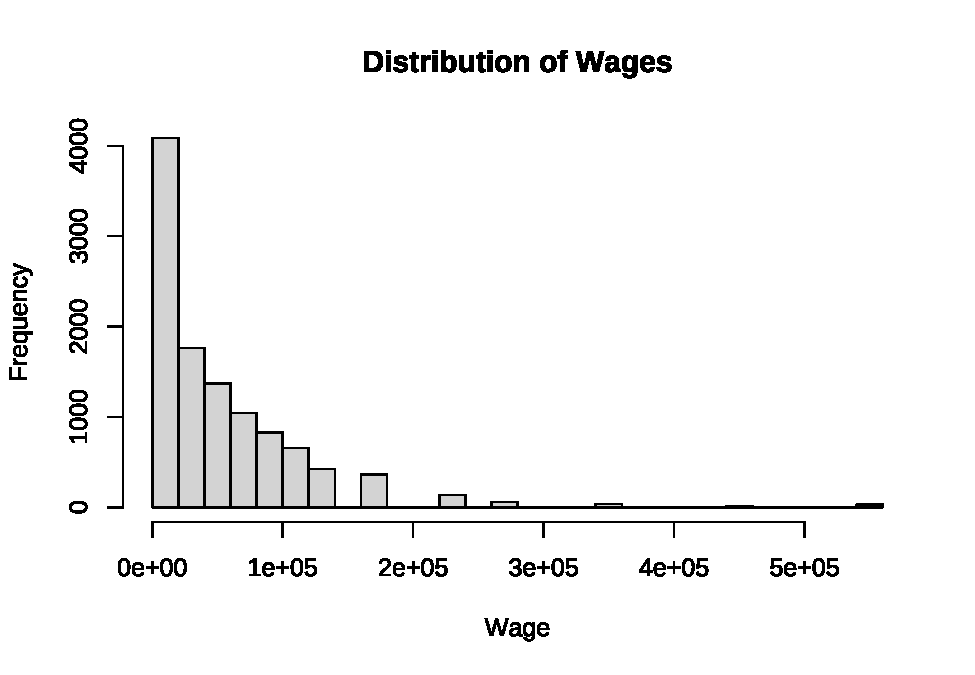
\includegraphics{Applied_Supervised_learning_Wage_prediction_Group_10_files/figure-latex/unnamed-chunk-2-1.pdf}

We have 10'711 observations with 78 variables like gender, age, country,
education, ecetera. We were then interested in getting a visual overview
of the most important data and the percentages.

Our aim was then to find the dependent variable (Y), in this case
`wage'.

\begin{Shaded}
\begin{Highlighting}[]
\CommentTok{\# Analyze the dependent variable \textquotesingle{}wage\textquotesingle{}}
\FunctionTok{summary}\NormalTok{(data\_wage}\SpecialCharTok{$}\NormalTok{wage)}
\end{Highlighting}
\end{Shaded}

\begin{verbatim}
##    Min. 1st Qu.  Median    Mean 3rd Qu.    Max. 
##       0    6811   34780   53048   75687  551774
\end{verbatim}

We can see that the average salary is over 52,300 dollars. As the
average wage is heavily distorted by high salaries - the maximum is
551,600 dollars - the median of just over 34,500 dollars is more
meaningful. Because the minimum value is zero, we were interested to see
how many people stated 0 as their salary (e.g.~students).

\begin{verbatim}
## Number of observations with zero wage: 1000
\end{verbatim}

This amounted to a total of 1000 people. we then created another dataset
without the people who entered 0 in the wage. The average value is
57,700 dollars, the median is 43,100 dollars.Additionally, we would like
to show the distribution of wages graphically.

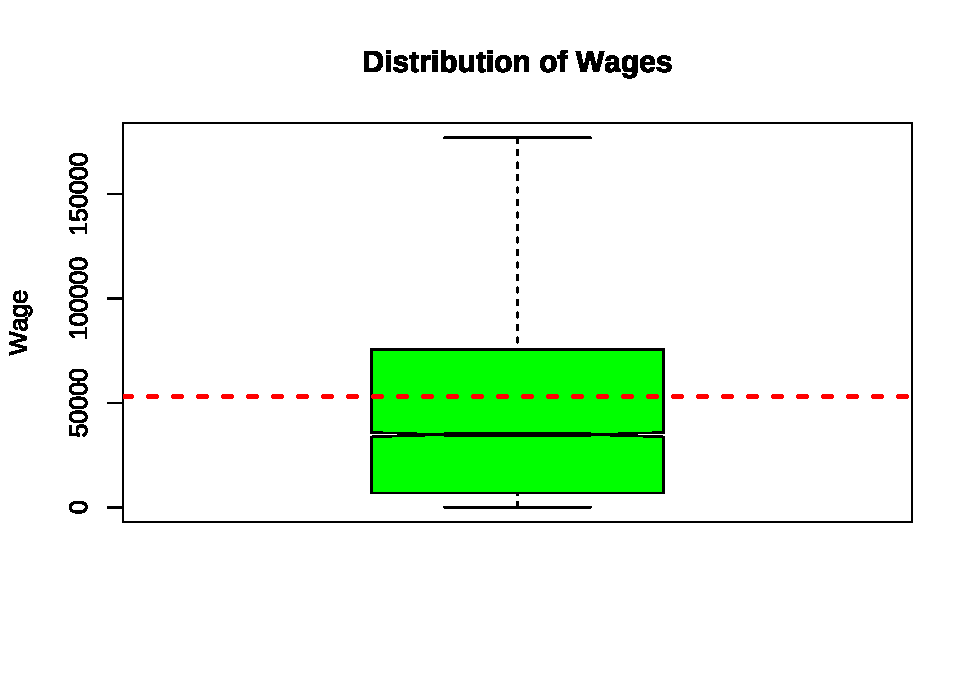
\includegraphics{Applied_Supervised_learning_Wage_prediction_Group_10_files/figure-latex/vizualising wage distribution-1.pdf}
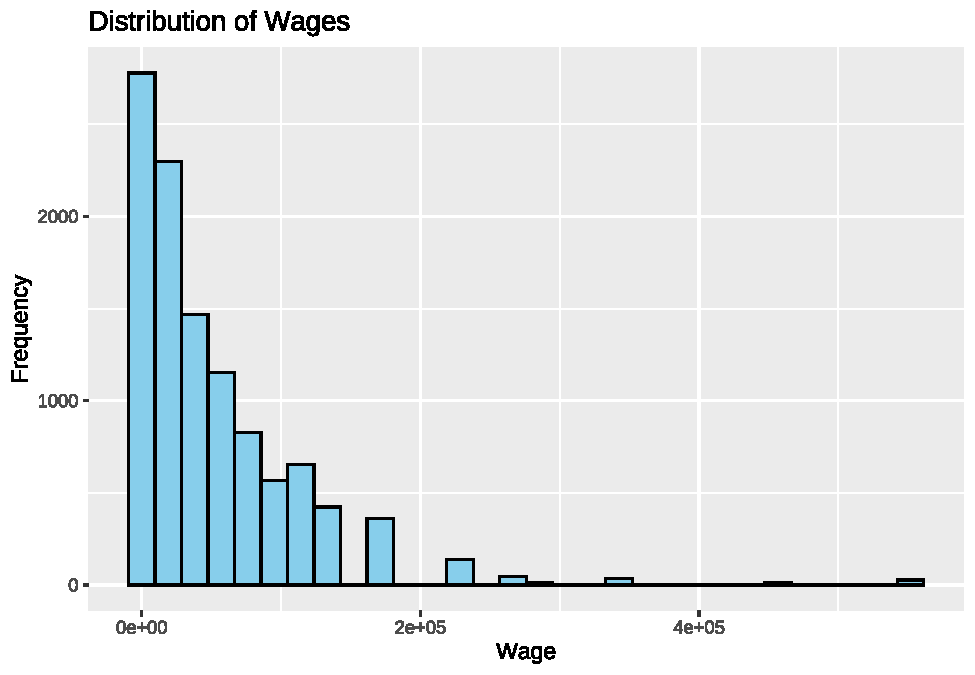
\includegraphics{Applied_Supervised_learning_Wage_prediction_Group_10_files/figure-latex/vizualising wage distribution-2.pdf}
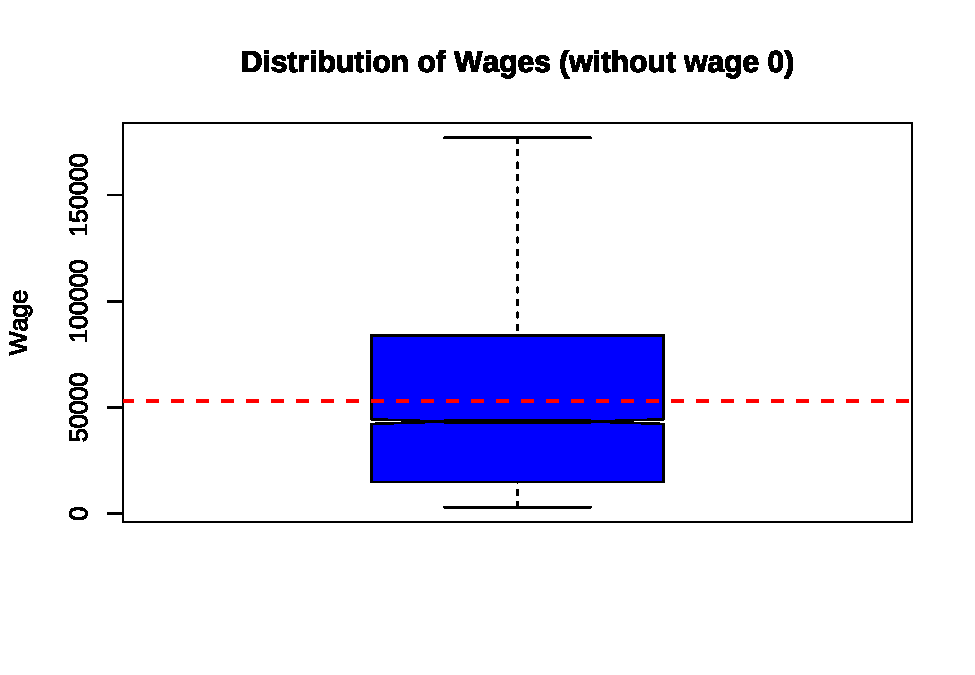
\includegraphics{Applied_Supervised_learning_Wage_prediction_Group_10_files/figure-latex/vizualising wage distribution-3.pdf}
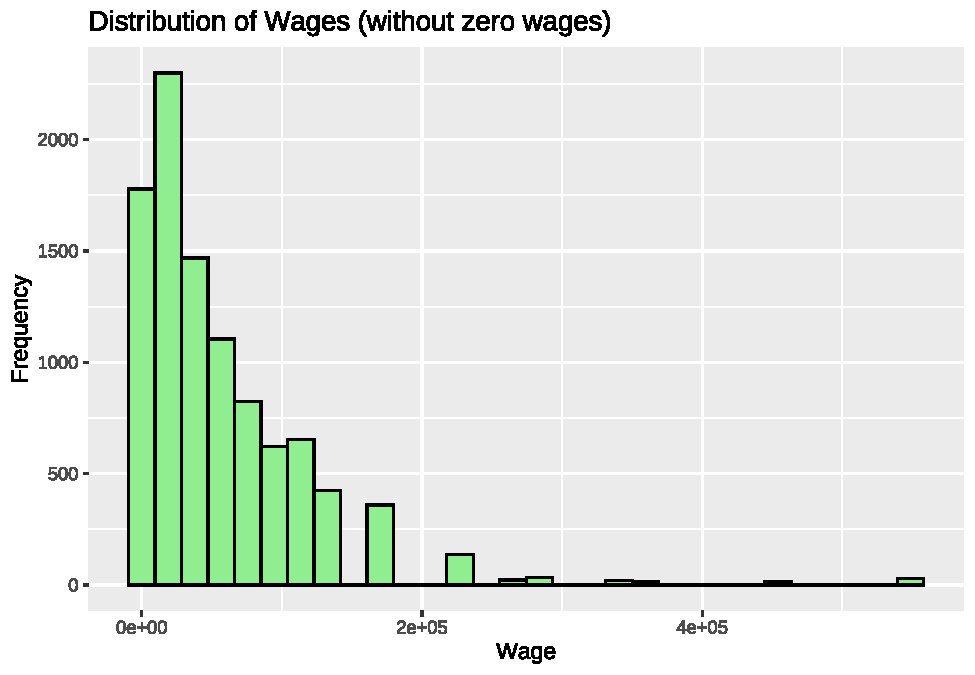
\includegraphics{Applied_Supervised_learning_Wage_prediction_Group_10_files/figure-latex/vizualising wage distribution-4.pdf}

It was relevant for us to work with the complete data (including all
upward outliers). On the other hand, we also work with the answers that
have a salary of 0. We believe that not to earn any money is also
relevant for our statistics. These could be people who are looking for a
job or students. This is also part of a prediction model for future
salaries.

We will then analyze the categorical and numerical values separately. By
looking at the data we found out, that only ``wage'' is a numeric
variable. That's why we then focused on the most important data besides
the wage: gender, age, experience, country, and education.

After these analyses, we concentrated on the top earners. In other
words, we looked for the top 5\% of earners.

\begin{verbatim}
## [1] 541  78
\end{verbatim}

\begin{verbatim}
##                  Female                    Male       Prefer not to say 
##                      38                     497                       4 
## Prefer to self-describe 
##                       2
\end{verbatim}

\begin{verbatim}
## 18-21 22-24 25-29 30-34 35-39 40-44 45-49 50-54 55-59 60-69 70-79   80+ 
##     3    18    52   106    82    70    78    55    42    33     2     0
\end{verbatim}

\begin{verbatim}
##   0-1   1-2   2-3   3-4   4-5  5-11 11-15 15-20 20-25 25-30  30 + 
##    46    38    41    33    46   101    90    53    42    24    27
\end{verbatim}

\begin{verbatim}
##                                            Argentina 
##                                                    0 
##                                            Australia 
##                                                   17 
##                                              Austria 
##                                                    0 
##                                           Bangladesh 
##                                                    0 
##                                              Belarus 
##                                                    0 
##                                              Belgium 
##                                                    1 
##                                               Brazil 
##                                                    6 
##                                               Canada 
##                                                   12 
##                                                Chile 
##                                                    1 
##                                                China 
##                                                    5 
##                                             Colombia 
##                                                    1 
##                                       Czech Republic 
##                                                    0 
##                                              Denmark 
##                                                    2 
##                                                Egypt 
##                                                    0 
##                                              Finland 
##                                                    0 
##                                               France 
##                                                    5 
##                                              Germany 
##                                                    4 
##                                               Greece 
##                                                    0 
##                                   Hong Kong (S.A.R.) 
##                                                    3 
##                                              Hungary 
##                                                    1 
##                I do not wish to disclose my location 
##                                                    2 
##                                                India 
##                                                   24 
##                                            Indonesia 
##                                                    1 
##                         Iran, Islamic Republic of... 
##                                                    0 
##                                              Ireland 
##                                                    1 
##                                               Israel 
##                                                    5 
##                                                Italy 
##                                                    0 
##                                                Japan 
##                                                    6 
##                                                Kenya 
##                                                    2 
##                                             Malaysia 
##                                                    0 
##                                               Mexico 
##                                                    0 
##                                              Morocco 
##                                                    0 
##                                          Netherlands 
##                                                    3 
##                                          New Zealand 
##                                                    0 
##                                              Nigeria 
##                                                    0 
##                                               Norway 
##                                                    0 
##                                                Other 
##                                                    6 
##                                             Pakistan 
##                                                    0 
##                                                 Peru 
##                                                    0 
##                                          Philippines 
##                                                    0 
##                                               Poland 
##                                                    0 
##                                             Portugal 
##                                                    0 
##                                    Republic of Korea 
##                                                    1 
##                                              Romania 
##                                                    0 
##                                               Russia 
##                                                    3 
##                                            Singapore 
##                                                    4 
##                                         South Africa 
##                                                    1 
##                                          South Korea 
##                                                    3 
##                                                Spain 
##                                                    1 
##                                               Sweden 
##                                                    1 
##                                          Switzerland 
##                                                   14 
##                                             Thailand 
##                                                    0 
##                                              Tunisia 
##                                                    1 
##                                               Turkey 
##                                                    0 
##                                              Ukraine 
##                                                    0 
## United Kingdom of Great Britain and Northern Ireland 
##                                                   18 
##                             United States of America 
##                                                  386 
##                                             Viet Nam 
##                                                    0
\end{verbatim}

\begin{verbatim}
##                                                 Bachelor’s degree 
##                                                                97 
##                                                   Doctoral degree 
##                                                               163 
##                                            I prefer not to answer 
##                                                                 2 
##                                                   Master’s degree 
##                                                               255 
##                                               Professional degree 
##                                                                13 
## Some college/university study without earning a bachelor’s degree 
##                                                                11
\end{verbatim}

We see that the top 5\% of the highest earners include a total of 536
people 491 men and 38 women. The analysis of the top 5\% shows that
people between the ages of 30 and 34 earn the most. In terms of
experience, it is people with between 5 and 11 years of work experience
who earn the most. 380 of the people come from the USA, which is no
surprise in this case, as most of the respondents come from the USA.
However, it is interesting to note that 255 of the 536 people have a
master's degree, while only 160 have a doctorate.

Then our goal was to scale numeric data to ensure that features have a
similar range of values. After that our goal was to convert categorical
variables into a format suitable for modeling.

\begin{Shaded}
\begin{Highlighting}[]
\CommentTok{\# Remove above all wages over 200\textquotesingle{}000}
\NormalTok{data\_wage }\OtherTok{\textless{}{-}}\NormalTok{ data\_wage }\SpecialCharTok{\%\textgreater{}\%} \FunctionTok{filter}\NormalTok{(wage }\SpecialCharTok{\textless{}=} \DecValTok{200000}\NormalTok{)}
\CommentTok{\# One{-}hot encode categorical variables and scale numeric variables}
\NormalTok{data\_encoded }\OtherTok{\textless{}{-}}\NormalTok{ data\_wage }\SpecialCharTok{\%\textgreater{}\%}
  \FunctionTok{mutate}\NormalTok{(}\FunctionTok{across}\NormalTok{(}\FunctionTok{where}\NormalTok{(is.character), factor)) }\SpecialCharTok{\%\textgreater{}\%}
  \FunctionTok{mutate}\NormalTok{(}\FunctionTok{across}\NormalTok{(}\FunctionTok{where}\NormalTok{(is.numeric), scale)) }\SpecialCharTok{\%\textgreater{}\%}
  \FunctionTok{mutate}\NormalTok{(}\FunctionTok{across}\NormalTok{(}\FunctionTok{where}\NormalTok{(is.factor), }\SpecialCharTok{\textasciitilde{}} \FunctionTok{as.numeric}\NormalTok{(}\FunctionTok{as.factor}\NormalTok{(.x)) }\SpecialCharTok{{-}} \DecValTok{1}\NormalTok{))}
\CommentTok{\# Add the target variable back to the transformed data}
\NormalTok{dummies }\OtherTok{\textless{}{-}} \FunctionTok{dummyVars}\NormalTok{(}\StringTok{" \textasciitilde{} ."}\NormalTok{, }\AttributeTok{data =}\NormalTok{ data\_encoded)}
\NormalTok{data\_transformed }\OtherTok{\textless{}{-}} \FunctionTok{as.data.frame}\NormalTok{(}\FunctionTok{predict}\NormalTok{(dummies, }\AttributeTok{newdata =}\NormalTok{ data\_encoded))}
\CommentTok{\# Add the target variable back}
\NormalTok{data\_transformed}\SpecialCharTok{$}\NormalTok{wage }\OtherTok{\textless{}{-}}\NormalTok{ data\_wage}\SpecialCharTok{$}\NormalTok{wage}
\end{Highlighting}
\end{Shaded}

Now it is time to decide which variables (characteristics) to include in
the model, based on their potential relationship to the target variable
``wage''.

\subsection{Model Selection and
Training:}\label{model-selection-and-training}

In this chapter we have trained different models (linear regression,
random forest, Generalized Boosted Regression Model (GBM) and xgboost)
in order to find the best performing one. The models were trained with
the data set data\_transformed.

\begin{Shaded}
\begin{Highlighting}[]
\CommentTok{\# Split data into training and testing sets}
\FunctionTok{set.seed}\NormalTok{(}\DecValTok{123}\NormalTok{)}
\NormalTok{split }\OtherTok{\textless{}{-}} \FunctionTok{initial\_split}\NormalTok{(data\_transformed, }\AttributeTok{prop =} \FloatTok{0.8}\NormalTok{)}
\NormalTok{train\_data }\OtherTok{\textless{}{-}} \FunctionTok{training}\NormalTok{(split)}
\NormalTok{test\_data }\OtherTok{\textless{}{-}} \FunctionTok{testing}\NormalTok{(split)}
\CommentTok{\# Helper function for model training and evaluation}
\NormalTok{train\_and\_evaluate\_model }\OtherTok{\textless{}{-}} \ControlFlowTok{function}\NormalTok{(model\_type, data) \{}
  \FunctionTok{set.seed}\NormalTok{(}\DecValTok{123}\NormalTok{)}
  \CommentTok{\# Define cross{-}validation method: Cross Validation with 5 folds means that the data is split into 5 parts, and the model is trained on 4 parts and tested on the 5th part. This process is repeated 5 times.}
\NormalTok{  train\_control }\OtherTok{\textless{}{-}} \FunctionTok{trainControl}\NormalTok{(}\AttributeTok{method =} \StringTok{"cv"}\NormalTok{, }\AttributeTok{number =} \DecValTok{5}\NormalTok{)}

  \ControlFlowTok{if}\NormalTok{ (model\_type }\SpecialCharTok{==} \StringTok{"xgbTree"}\NormalTok{) \{}
\NormalTok{    data\_no\_wage }\OtherTok{\textless{}{-}}\NormalTok{ data[, }\SpecialCharTok{!}\FunctionTok{names}\NormalTok{(data) }\SpecialCharTok{\%in\%} \StringTok{"wage"}\NormalTok{]}
\NormalTok{    model }\OtherTok{\textless{}{-}} \FunctionTok{train}\NormalTok{(}
      \AttributeTok{x =}\NormalTok{ data\_no\_wage,}
      \AttributeTok{y =}\NormalTok{ data}\SpecialCharTok{$}\NormalTok{wage,}
      \AttributeTok{method =}\NormalTok{ model\_type,}
      \AttributeTok{trControl =}\NormalTok{ train\_control,}
      \AttributeTok{tuneLength =} \DecValTok{3}
\NormalTok{    )}
\NormalTok{  \} }\ControlFlowTok{else}\NormalTok{ \{}
\NormalTok{    model }\OtherTok{\textless{}{-}} \FunctionTok{train}\NormalTok{(}
\NormalTok{      wage }\SpecialCharTok{\textasciitilde{}}\NormalTok{ .,}
      \AttributeTok{data =}\NormalTok{ data,}
      \AttributeTok{method =}\NormalTok{ model\_type,}
      \AttributeTok{trControl =}\NormalTok{ train\_control}
\NormalTok{    )}
\NormalTok{  \}}
  \FunctionTok{return}\NormalTok{(model)}
\NormalTok{\}}
\CommentTok{\# Train models}
\NormalTok{lm\_model }\OtherTok{\textless{}{-}} \FunctionTok{train\_and\_evaluate\_model}\NormalTok{(}\StringTok{"lm"}\NormalTok{, train\_data)}
\CommentTok{\# We have to use the randomForest package for the random forest model and not the train\_and\_evaluate\_model function otherwise  varImpPlot will throw an type error.}
\NormalTok{rf\_model }\OtherTok{\textless{}{-}} \FunctionTok{randomForest}\NormalTok{(}
\NormalTok{  wage }\SpecialCharTok{\textasciitilde{}}\NormalTok{ .,}
  \AttributeTok{data =}\NormalTok{ train\_data, }\AttributeTok{ntree =} \DecValTok{50}\NormalTok{, }\AttributeTok{mtry =} \DecValTok{3}\NormalTok{, }\AttributeTok{importance =} \ConstantTok{TRUE}\NormalTok{, }\AttributeTok{cp =} \DecValTok{0}
\NormalTok{)}
\NormalTok{gbm\_model }\OtherTok{\textless{}{-}} \FunctionTok{train\_and\_evaluate\_model}\NormalTok{(}\StringTok{"gbm"}\NormalTok{, train\_data)}
\end{Highlighting}
\end{Shaded}

\begin{verbatim}
## Iter   TrainDeviance   ValidDeviance   StepSize   Improve
##      1 1976689875.6334             nan     0.1000 91399438.8225
##      2 1901206912.9915             nan     0.1000 75586690.1023
##      3 1833375533.2110             nan     0.1000 68249657.3525
##      4 1769329636.5547             nan     0.1000 60302547.0438
##      5 1714852903.9282             nan     0.1000 54251217.2705
##      6 1666773528.4568             nan     0.1000 47082714.1406
##      7 1624660664.4980             nan     0.1000 43388155.4000
##      8 1583566262.0740             nan     0.1000 38956160.9005
##      9 1547693204.4281             nan     0.1000 34423458.1417
##     10 1515861791.2758             nan     0.1000 31542646.5695
##     20 1290066096.9378             nan     0.1000 15216401.1429
##     40 1095737272.8344             nan     0.1000 5448841.1908
##     60 1017596706.1537             nan     0.1000 2044394.0413
##     80 974513432.6662             nan     0.1000 1675678.3538
##    100 946777711.6091             nan     0.1000 390895.1476
##    120 928008413.2429             nan     0.1000 308397.5164
##    140 914244013.2058             nan     0.1000 218681.8003
##    150 908864959.5827             nan     0.1000 -226737.5689
## 
## Iter   TrainDeviance   ValidDeviance   StepSize   Improve
##      1 1937360771.2621             nan     0.1000 128603116.0921
##      2 1831370837.6841             nan     0.1000 107706707.4066
##      3 1740514804.7992             nan     0.1000 93796663.6530
##      4 1661229251.3373             nan     0.1000 76702027.0828
##      5 1586191493.7106             nan     0.1000 75451870.0038
##      6 1525857890.3020             nan     0.1000 59681100.6940
##      7 1472415552.4707             nan     0.1000 54542808.5805
##      8 1418544836.2718             nan     0.1000 51344629.6647
##      9 1378066771.2800             nan     0.1000 41083290.0854
##     10 1332331505.2030             nan     0.1000 43546007.7324
##     20 1105085071.4079             nan     0.1000 13228339.7027
##     40 941124335.6551             nan     0.1000 4523414.7591
##     60 876881210.8053             nan     0.1000 3248363.8156
##     80 840705272.8316             nan     0.1000 2538900.6011
##    100 817279154.0451             nan     0.1000 857795.6036
##    120 802865394.4557             nan     0.1000 266136.7550
##    140 786267028.3002             nan     0.1000 437711.6611
##    150 780193263.9584             nan     0.1000 -330637.0863
## 
## Iter   TrainDeviance   ValidDeviance   StepSize   Improve
##      1 1914077878.7866             nan     0.1000 158174875.6355
##      2 1777414852.5675             nan     0.1000 134652797.7585
##      3 1666865382.1763             nan     0.1000 109130959.3316
##      4 1576320406.0135             nan     0.1000 86287472.3704
##      5 1501315360.7826             nan     0.1000 74868097.9396
##      6 1439540296.2249             nan     0.1000 62924329.8036
##      7 1388151121.2484             nan     0.1000 53150883.1672
##      8 1337311182.2403             nan     0.1000 49075131.3331
##      9 1294826717.5713             nan     0.1000 38893895.8307
##     10 1261022701.8212             nan     0.1000 33374507.7458
##     20 1034024102.2024             nan     0.1000 12442048.0852
##     40 883256742.1885             nan     0.1000 4148240.8697
##     60 820836765.6536             nan     0.1000 302991.9718
##     80 787082488.1971             nan     0.1000 847391.7834
##    100 762939788.3305             nan     0.1000 1543287.5961
##    120 744775705.3829             nan     0.1000 -442555.0532
##    140 728478013.0523             nan     0.1000 42679.8294
##    150 722656729.7371             nan     0.1000 120499.6015
## 
## Iter   TrainDeviance   ValidDeviance   StepSize   Improve
##      1 1974374485.7976             nan     0.1000 92073314.1659
##      2 1895612447.1709             nan     0.1000 78331412.3718
##      3 1828072807.8536             nan     0.1000 67288679.7678
##      4 1766561014.2867             nan     0.1000 60100405.0016
##      5 1712300347.2714             nan     0.1000 53755475.7937
##      6 1661603779.0198             nan     0.1000 46885289.9524
##      7 1621712592.5153             nan     0.1000 40557305.5751
##      8 1580984164.3226             nan     0.1000 40142318.4638
##      9 1544218637.5259             nan     0.1000 37656433.0568
##     10 1510953709.9574             nan     0.1000 32345872.5203
##     20 1283879732.0422             nan     0.1000 14564316.4225
##     40 1092834358.1210             nan     0.1000 4268427.7850
##     60 1013691722.4889             nan     0.1000 1949795.5476
##     80 970169506.4551             nan     0.1000 1144981.9060
##    100 942818086.3417             nan     0.1000 228533.5365
##    120 923276528.3536             nan     0.1000 744879.9679
##    140 909433487.6698             nan     0.1000 -100780.7685
##    150 903450292.7437             nan     0.1000 326345.3597
## 
## Iter   TrainDeviance   ValidDeviance   StepSize   Improve
##      1 1934053242.0442             nan     0.1000 131034813.6593
##      2 1829430431.3639             nan     0.1000 106610762.8620
##      3 1740643045.4972             nan     0.1000 90481811.3185
##      4 1661689797.8941             nan     0.1000 74700269.2842
##      5 1599256916.7798             nan     0.1000 63376465.4367
##      6 1533088737.1046             nan     0.1000 65736080.2779
##      7 1478204656.7299             nan     0.1000 50589290.5271
##      8 1427098913.5363             nan     0.1000 50972153.8903
##      9 1384187726.5732             nan     0.1000 41408758.1728
##     10 1350348883.8102             nan     0.1000 34470644.3116
##     20 1112701636.0059             nan     0.1000 15341767.0933
##     40 946575625.8897             nan     0.1000 4159451.3325
##     60 879976410.8546             nan     0.1000 3278027.7458
##     80 842180721.4672             nan     0.1000 853978.8001
##    100 820538750.8407             nan     0.1000 419324.5882
##    120 798359125.1487             nan     0.1000 95693.0718
##    140 782274553.2948             nan     0.1000 -114662.2204
##    150 774534067.9645             nan     0.1000 538576.0373
## 
## Iter   TrainDeviance   ValidDeviance   StepSize   Improve
##      1 1905814624.3307             nan     0.1000 154775794.7375
##      2 1777710140.3362             nan     0.1000 127568644.6546
##      3 1667356669.2646             nan     0.1000 104690804.0478
##      4 1582045091.6013             nan     0.1000 83804753.9108
##      5 1506362020.6954             nan     0.1000 72904749.9689
##      6 1446568833.0802             nan     0.1000 57725826.8880
##      7 1393836719.2226             nan     0.1000 54364844.1738
##      8 1348011859.7573             nan     0.1000 47110148.4939
##      9 1307430324.8116             nan     0.1000 38769499.0291
##     10 1271970002.0283             nan     0.1000 33836447.4033
##     20 1049635435.4812             nan     0.1000 13164223.6317
##     40 882461410.2462             nan     0.1000 5113869.5777
##     60 826379481.6270             nan     0.1000 521650.2901
##     80 795484424.6173             nan     0.1000 -364943.7732
##    100 767861619.7570             nan     0.1000 287031.0537
##    120 744308766.3969             nan     0.1000 -176558.3921
##    140 724970815.4984             nan     0.1000 -572777.4913
##    150 716735414.0833             nan     0.1000 -659177.5521
## 
## Iter   TrainDeviance   ValidDeviance   StepSize   Improve
##      1 1953473148.1391             nan     0.1000 93497631.3985
##      2 1879501256.4275             nan     0.1000 75341518.3485
##      3 1812432404.4552             nan     0.1000 66958501.5488
##      4 1751848718.0144             nan     0.1000 61426037.8131
##      5 1700885377.8724             nan     0.1000 51734423.9718
##      6 1647127590.0843             nan     0.1000 52515298.0401
##      7 1605307443.7273             nan     0.1000 40103310.8351
##      8 1562889201.8897             nan     0.1000 41993343.4982
##      9 1529069165.9419             nan     0.1000 32227550.2442
##     10 1495928748.5416             nan     0.1000 33377568.8941
##     20 1274161577.9056             nan     0.1000 15175092.8072
##     40 1081067214.0155             nan     0.1000 4786319.5606
##     60 1004537929.0199             nan     0.1000 2784776.1307
##     80 960139764.5729             nan     0.1000 1143700.5394
##    100 931394077.7601             nan     0.1000 943285.0185
##    120 911035000.4080             nan     0.1000 972010.3903
##    140 896280290.2121             nan     0.1000 68432.5106
##    150 890028238.3229             nan     0.1000 -378676.6585
## 
## Iter   TrainDeviance   ValidDeviance   StepSize   Improve
##      1 1915753031.9677             nan     0.1000 131286211.8194
##      2 1809587893.0719             nan     0.1000 109276987.9177
##      3 1721705542.9620             nan     0.1000 89185247.9555
##      4 1638486916.6903             nan     0.1000 85537487.4184
##      5 1574772192.5563             nan     0.1000 66286548.8609
##      6 1517376649.6319             nan     0.1000 58489915.2303
##      7 1463083369.3619             nan     0.1000 54097026.2902
##      8 1410331977.7045             nan     0.1000 53272358.8273
##      9 1368581630.8969             nan     0.1000 40293104.4071
##     10 1323168627.4273             nan     0.1000 43941883.4424
##     20 1090604782.5786             nan     0.1000 16153598.9423
##     40 933594338.3755             nan     0.1000 3726910.4300
##     60 865652431.6962             nan     0.1000 453322.6708
##     80 829314640.4113             nan     0.1000 1592071.9520
##    100 804602856.6902             nan     0.1000 1353146.2628
##    120 784768620.0288             nan     0.1000 -383811.9255
##    140 771029137.4635             nan     0.1000 436023.7787
##    150 764544441.3831             nan     0.1000 367349.1182
## 
## Iter   TrainDeviance   ValidDeviance   StepSize   Improve
##      1 1884600617.0781             nan     0.1000 155646677.8218
##      2 1761695929.9058             nan     0.1000 124864574.7673
##      3 1651573159.6777             nan     0.1000 108713251.7366
##      4 1564368497.2720             nan     0.1000 85615160.6628
##      5 1490146417.1564             nan     0.1000 72086481.5653
##      6 1428888763.7935             nan     0.1000 61009811.0871
##      7 1377267331.2505             nan     0.1000 49867925.9966
##      8 1331471933.8373             nan     0.1000 43885563.0255
##      9 1291777264.0169             nan     0.1000 39253438.9517
##     10 1254604462.0572             nan     0.1000 37475198.1524
##     20 1035616708.8049             nan     0.1000 12092101.0425
##     40 877740020.9230             nan     0.1000 4124882.7692
##     60 816666553.2810             nan     0.1000 987605.5597
##     80 784017136.8424             nan     0.1000 212229.2477
##    100 756645005.1582             nan     0.1000 -24043.5769
##    120 732282951.5883             nan     0.1000 587655.6059
##    140 715555210.3815             nan     0.1000 770215.6798
##    150 706335769.5029             nan     0.1000 30304.9968
## 
## Iter   TrainDeviance   ValidDeviance   StepSize   Improve
##      1 1973099681.1420             nan     0.1000 94937346.9037
##      2 1891921242.7717             nan     0.1000 76993550.1472
##      3 1825384291.8280             nan     0.1000 66981776.8336
##      4 1764123657.3092             nan     0.1000 58713050.9242
##      5 1712637442.2289             nan     0.1000 53756308.3142
##      6 1667058258.5850             nan     0.1000 43447731.1020
##      7 1621638652.1430             nan     0.1000 46927562.0827
##      8 1582272319.6041             nan     0.1000 39597377.5896
##      9 1545296639.4765             nan     0.1000 34544017.7516
##     10 1511854842.1337             nan     0.1000 34215879.3583
##     20 1281933972.1238             nan     0.1000 18222222.7126
##     40 1077895928.8225             nan     0.1000 6573736.8933
##     60 999546778.0521             nan     0.1000 2387752.5886
##     80 954468343.6622             nan     0.1000 941418.6643
##    100 926076490.5503             nan     0.1000 894461.1735
##    120 906633729.9669             nan     0.1000 627672.6881
##    140 891511651.4977             nan     0.1000 474665.8316
##    150 885376890.8097             nan     0.1000 314324.5747
## 
## Iter   TrainDeviance   ValidDeviance   StepSize   Improve
##      1 1934563903.3200             nan     0.1000 129026862.8863
##      2 1829749993.2403             nan     0.1000 107677827.8175
##      3 1735028250.7766             nan     0.1000 89210721.0906
##      4 1650485033.6835             nan     0.1000 82549875.2653
##      5 1583161421.2772             nan     0.1000 67091722.5286
##      6 1521844428.1177             nan     0.1000 62719225.4589
##      7 1473047911.6609             nan     0.1000 47324611.8432
##      8 1424111173.7000             nan     0.1000 49209891.4043
##      9 1375993029.2989             nan     0.1000 48306017.1962
##     10 1329192038.6221             nan     0.1000 44197339.0832
##     20 1092872004.3425             nan     0.1000 12410154.8204
##     40 925689960.9912             nan     0.1000 3163979.3699
##     60 854298633.7239             nan     0.1000 2082374.0325
##     80 817242710.3539             nan     0.1000 570846.9216
##    100 796724395.6383             nan     0.1000 223132.9608
##    120 778529825.3136             nan     0.1000 270956.4552
##    140 763094838.0489             nan     0.1000 96205.0108
##    150 755843146.1533             nan     0.1000 -116862.0955
## 
## Iter   TrainDeviance   ValidDeviance   StepSize   Improve
##      1 1905191346.6862             nan     0.1000 157831350.8522
##      2 1773192931.1584             nan     0.1000 129729282.9183
##      3 1667077897.0467             nan     0.1000 104069273.0922
##      4 1579290334.3743             nan     0.1000 84309953.4414
##      5 1501479460.7164             nan     0.1000 78926555.8863
##      6 1435383956.4138             nan     0.1000 59737771.3770
##      7 1384289260.2317             nan     0.1000 50787367.7025
##      8 1338944147.7806             nan     0.1000 42905799.6744
##      9 1295494278.9317             nan     0.1000 42484774.2628
##     10 1257682104.0199             nan     0.1000 37318080.9043
##     20 1024880483.6924             nan     0.1000 14493252.1148
##     40 863097498.5732             nan     0.1000 2133836.7024
##     60 802803594.2961             nan     0.1000 53912.6291
##     80 771584110.3695             nan     0.1000 365191.6631
##    100 745080047.2756             nan     0.1000 -29333.6075
##    120 722940344.4776             nan     0.1000 373520.0397
##    140 709080806.7379             nan     0.1000 315648.7434
##    150 701586067.2830             nan     0.1000 44561.8185
## 
## Iter   TrainDeviance   ValidDeviance   StepSize   Improve
##      1 1954315141.8432             nan     0.1000 89493826.7402
##      2 1883782820.7884             nan     0.1000 70955738.5165
##      3 1807060626.2477             nan     0.1000 73567778.0016
##      4 1750056801.1189             nan     0.1000 59098083.1663
##      5 1694259177.6437             nan     0.1000 55310631.9137
##      6 1643614792.7141             nan     0.1000 49018435.4285
##      7 1600233209.7896             nan     0.1000 44372071.6563
##      8 1563580351.0308             nan     0.1000 35927298.8000
##      9 1529072911.5136             nan     0.1000 33723426.7476
##     10 1491857845.9547             nan     0.1000 36986344.9951
##     20 1267014390.8709             nan     0.1000 14025311.2656
##     40 1076036107.6775             nan     0.1000 5437889.6803
##     60 1001972283.7162             nan     0.1000 2269687.4434
##     80 958686883.1844             nan     0.1000 999711.5924
##    100 931208469.3765             nan     0.1000 844249.8413
##    120 910937785.5109             nan     0.1000 788226.4967
##    140 896346041.3732             nan     0.1000 452013.0343
##    150 890446750.0487             nan     0.1000 260419.0841
## 
## Iter   TrainDeviance   ValidDeviance   StepSize   Improve
##      1 1913975161.4080             nan     0.1000 127398681.8404
##      2 1812179790.4583             nan     0.1000 103301169.2784
##      3 1723758159.0778             nan     0.1000 87526418.4469
##      4 1644530115.7301             nan     0.1000 74817439.2943
##      5 1570317109.5783             nan     0.1000 75277407.7293
##      6 1507368829.7722             nan     0.1000 59995877.8493
##      7 1455254436.2331             nan     0.1000 50265665.8332
##      8 1403384106.7017             nan     0.1000 52068149.4817
##      9 1361295984.8192             nan     0.1000 41959293.8042
##     10 1323480967.3669             nan     0.1000 34622695.4497
##     20 1094692557.5249             nan     0.1000 13677314.2824
##     40 934169396.7656             nan     0.1000 4401256.8850
##     60 869205872.5980             nan     0.1000 2780786.7168
##     80 833625900.1324             nan     0.1000 -196826.4654
##    100 809546737.3126             nan     0.1000 -626258.0232
##    120 793223189.9157             nan     0.1000 101622.7659
##    140 773010949.0732             nan     0.1000 265138.9331
##    150 767129330.8767             nan     0.1000 -75768.1252
## 
## Iter   TrainDeviance   ValidDeviance   StepSize   Improve
##      1 1887075312.9642             nan     0.1000 151953840.0146
##      2 1757719191.6806             nan     0.1000 126112472.9819
##      3 1650825680.2117             nan     0.1000 102196783.7491
##      4 1564686152.9381             nan     0.1000 89164320.1642
##      5 1491791159.4577             nan     0.1000 69729520.2260
##      6 1427380576.5345             nan     0.1000 61072758.9348
##      7 1374552002.2587             nan     0.1000 51490764.6422
##      8 1325245497.5050             nan     0.1000 46093188.1087
##      9 1289031917.0510             nan     0.1000 35937019.1726
##     10 1255621824.1816             nan     0.1000 34671911.7118
##     20 1035098820.0987             nan     0.1000 12046949.1573
##     40 876814768.1178             nan     0.1000 4838039.2033
##     60 818301192.2111             nan     0.1000 2386139.7864
##     80 780234724.3043             nan     0.1000 -211332.1727
##    100 754319056.8045             nan     0.1000 -279320.5431
##    120 738392979.3806             nan     0.1000 -189824.4351
##    140 719830336.0742             nan     0.1000 -92351.3615
##    150 709857307.6148             nan     0.1000 -19776.4809
## 
## Iter   TrainDeviance   ValidDeviance   StepSize   Improve
##      1 1904944340.6765             nan     0.1000 154538826.4794
##      2 1771515387.3861             nan     0.1000 132116606.4476
##      3 1666424350.2388             nan     0.1000 103426985.4133
##      4 1578760386.0896             nan     0.1000 87649748.8332
##      5 1504362998.1970             nan     0.1000 72763903.6077
##      6 1441721990.0903             nan     0.1000 60212678.3151
##      7 1386731210.3084             nan     0.1000 54443821.3772
##      8 1342069029.6335             nan     0.1000 43461354.4857
##      9 1297522380.1361             nan     0.1000 44529992.3530
##     10 1262737991.5176             nan     0.1000 35038843.2280
##     20 1037186094.0635             nan     0.1000 14748124.1121
##     40 878648361.5825             nan     0.1000 2645764.4513
##     60 817378316.3809             nan     0.1000 2419975.0039
##     80 785831497.4742             nan     0.1000 358979.7383
##    100 763747298.6222             nan     0.1000 -162653.3433
##    120 741396193.5411             nan     0.1000 1802618.0801
##    140 727393099.8811             nan     0.1000 411862.8284
##    150 718162672.1414             nan     0.1000 -97748.9810
\end{verbatim}

\begin{Shaded}
\begin{Highlighting}[]
\NormalTok{xgboost\_model }\OtherTok{\textless{}{-}} \FunctionTok{train\_and\_evaluate\_model}\NormalTok{(}\StringTok{"xgbTree"}\NormalTok{, train\_data)}
\end{Highlighting}
\end{Shaded}

\begin{verbatim}
## [14:18:59] WARNING: src/c_api/c_api.cc:935: `ntree_limit` is deprecated, use `iteration_range` instead.
## [14:18:59] WARNING: src/c_api/c_api.cc:935: `ntree_limit` is deprecated, use `iteration_range` instead.
## [14:18:59] WARNING: src/c_api/c_api.cc:935: `ntree_limit` is deprecated, use `iteration_range` instead.
## [14:18:59] WARNING: src/c_api/c_api.cc:935: `ntree_limit` is deprecated, use `iteration_range` instead.
## [14:19:00] WARNING: src/c_api/c_api.cc:935: `ntree_limit` is deprecated, use `iteration_range` instead.
## [14:19:00] WARNING: src/c_api/c_api.cc:935: `ntree_limit` is deprecated, use `iteration_range` instead.
## [14:19:00] WARNING: src/c_api/c_api.cc:935: `ntree_limit` is deprecated, use `iteration_range` instead.
## [14:19:00] WARNING: src/c_api/c_api.cc:935: `ntree_limit` is deprecated, use `iteration_range` instead.
## [14:19:01] WARNING: src/c_api/c_api.cc:935: `ntree_limit` is deprecated, use `iteration_range` instead.
## [14:19:01] WARNING: src/c_api/c_api.cc:935: `ntree_limit` is deprecated, use `iteration_range` instead.
## [14:19:01] WARNING: src/c_api/c_api.cc:935: `ntree_limit` is deprecated, use `iteration_range` instead.
## [14:19:01] WARNING: src/c_api/c_api.cc:935: `ntree_limit` is deprecated, use `iteration_range` instead.
## [14:19:02] WARNING: src/c_api/c_api.cc:935: `ntree_limit` is deprecated, use `iteration_range` instead.
## [14:19:02] WARNING: src/c_api/c_api.cc:935: `ntree_limit` is deprecated, use `iteration_range` instead.
## [14:19:03] WARNING: src/c_api/c_api.cc:935: `ntree_limit` is deprecated, use `iteration_range` instead.
## [14:19:03] WARNING: src/c_api/c_api.cc:935: `ntree_limit` is deprecated, use `iteration_range` instead.
## [14:19:03] WARNING: src/c_api/c_api.cc:935: `ntree_limit` is deprecated, use `iteration_range` instead.
## [14:19:03] WARNING: src/c_api/c_api.cc:935: `ntree_limit` is deprecated, use `iteration_range` instead.
## [14:19:04] WARNING: src/c_api/c_api.cc:935: `ntree_limit` is deprecated, use `iteration_range` instead.
## [14:19:04] WARNING: src/c_api/c_api.cc:935: `ntree_limit` is deprecated, use `iteration_range` instead.
## [14:19:05] WARNING: src/c_api/c_api.cc:935: `ntree_limit` is deprecated, use `iteration_range` instead.
## [14:19:05] WARNING: src/c_api/c_api.cc:935: `ntree_limit` is deprecated, use `iteration_range` instead.
## [14:19:06] WARNING: src/c_api/c_api.cc:935: `ntree_limit` is deprecated, use `iteration_range` instead.
## [14:19:06] WARNING: src/c_api/c_api.cc:935: `ntree_limit` is deprecated, use `iteration_range` instead.
## [14:19:07] WARNING: src/c_api/c_api.cc:935: `ntree_limit` is deprecated, use `iteration_range` instead.
## [14:19:07] WARNING: src/c_api/c_api.cc:935: `ntree_limit` is deprecated, use `iteration_range` instead.
## [14:19:08] WARNING: src/c_api/c_api.cc:935: `ntree_limit` is deprecated, use `iteration_range` instead.
## [14:19:08] WARNING: src/c_api/c_api.cc:935: `ntree_limit` is deprecated, use `iteration_range` instead.
## [14:19:09] WARNING: src/c_api/c_api.cc:935: `ntree_limit` is deprecated, use `iteration_range` instead.
## [14:19:09] WARNING: src/c_api/c_api.cc:935: `ntree_limit` is deprecated, use `iteration_range` instead.
## [14:19:11] WARNING: src/c_api/c_api.cc:935: `ntree_limit` is deprecated, use `iteration_range` instead.
## [14:19:11] WARNING: src/c_api/c_api.cc:935: `ntree_limit` is deprecated, use `iteration_range` instead.
## [14:19:12] WARNING: src/c_api/c_api.cc:935: `ntree_limit` is deprecated, use `iteration_range` instead.
## [14:19:12] WARNING: src/c_api/c_api.cc:935: `ntree_limit` is deprecated, use `iteration_range` instead.
## [14:19:13] WARNING: src/c_api/c_api.cc:935: `ntree_limit` is deprecated, use `iteration_range` instead.
## [14:19:13] WARNING: src/c_api/c_api.cc:935: `ntree_limit` is deprecated, use `iteration_range` instead.
## [14:19:14] WARNING: src/c_api/c_api.cc:935: `ntree_limit` is deprecated, use `iteration_range` instead.
## [14:19:14] WARNING: src/c_api/c_api.cc:935: `ntree_limit` is deprecated, use `iteration_range` instead.
## [14:19:14] WARNING: src/c_api/c_api.cc:935: `ntree_limit` is deprecated, use `iteration_range` instead.
## [14:19:14] WARNING: src/c_api/c_api.cc:935: `ntree_limit` is deprecated, use `iteration_range` instead.
## [14:19:14] WARNING: src/c_api/c_api.cc:935: `ntree_limit` is deprecated, use `iteration_range` instead.
## [14:19:14] WARNING: src/c_api/c_api.cc:935: `ntree_limit` is deprecated, use `iteration_range` instead.
## [14:19:15] WARNING: src/c_api/c_api.cc:935: `ntree_limit` is deprecated, use `iteration_range` instead.
## [14:19:15] WARNING: src/c_api/c_api.cc:935: `ntree_limit` is deprecated, use `iteration_range` instead.
## [14:19:15] WARNING: src/c_api/c_api.cc:935: `ntree_limit` is deprecated, use `iteration_range` instead.
## [14:19:15] WARNING: src/c_api/c_api.cc:935: `ntree_limit` is deprecated, use `iteration_range` instead.
## [14:19:16] WARNING: src/c_api/c_api.cc:935: `ntree_limit` is deprecated, use `iteration_range` instead.
## [14:19:16] WARNING: src/c_api/c_api.cc:935: `ntree_limit` is deprecated, use `iteration_range` instead.
## [14:19:17] WARNING: src/c_api/c_api.cc:935: `ntree_limit` is deprecated, use `iteration_range` instead.
## [14:19:17] WARNING: src/c_api/c_api.cc:935: `ntree_limit` is deprecated, use `iteration_range` instead.
## [14:19:17] WARNING: src/c_api/c_api.cc:935: `ntree_limit` is deprecated, use `iteration_range` instead.
## [14:19:17] WARNING: src/c_api/c_api.cc:935: `ntree_limit` is deprecated, use `iteration_range` instead.
## [14:19:18] WARNING: src/c_api/c_api.cc:935: `ntree_limit` is deprecated, use `iteration_range` instead.
## [14:19:18] WARNING: src/c_api/c_api.cc:935: `ntree_limit` is deprecated, use `iteration_range` instead.
## [14:19:19] WARNING: src/c_api/c_api.cc:935: `ntree_limit` is deprecated, use `iteration_range` instead.
## [14:19:19] WARNING: src/c_api/c_api.cc:935: `ntree_limit` is deprecated, use `iteration_range` instead.
## [14:19:20] WARNING: src/c_api/c_api.cc:935: `ntree_limit` is deprecated, use `iteration_range` instead.
## [14:19:20] WARNING: src/c_api/c_api.cc:935: `ntree_limit` is deprecated, use `iteration_range` instead.
## [14:19:21] WARNING: src/c_api/c_api.cc:935: `ntree_limit` is deprecated, use `iteration_range` instead.
## [14:19:21] WARNING: src/c_api/c_api.cc:935: `ntree_limit` is deprecated, use `iteration_range` instead.
## [14:19:22] WARNING: src/c_api/c_api.cc:935: `ntree_limit` is deprecated, use `iteration_range` instead.
## [14:19:22] WARNING: src/c_api/c_api.cc:935: `ntree_limit` is deprecated, use `iteration_range` instead.
## [14:19:23] WARNING: src/c_api/c_api.cc:935: `ntree_limit` is deprecated, use `iteration_range` instead.
## [14:19:23] WARNING: src/c_api/c_api.cc:935: `ntree_limit` is deprecated, use `iteration_range` instead.
## [14:19:24] WARNING: src/c_api/c_api.cc:935: `ntree_limit` is deprecated, use `iteration_range` instead.
## [14:19:24] WARNING: src/c_api/c_api.cc:935: `ntree_limit` is deprecated, use `iteration_range` instead.
## [14:19:25] WARNING: src/c_api/c_api.cc:935: `ntree_limit` is deprecated, use `iteration_range` instead.
## [14:19:25] WARNING: src/c_api/c_api.cc:935: `ntree_limit` is deprecated, use `iteration_range` instead.
## [14:19:27] WARNING: src/c_api/c_api.cc:935: `ntree_limit` is deprecated, use `iteration_range` instead.
## [14:19:27] WARNING: src/c_api/c_api.cc:935: `ntree_limit` is deprecated, use `iteration_range` instead.
## [14:19:28] WARNING: src/c_api/c_api.cc:935: `ntree_limit` is deprecated, use `iteration_range` instead.
## [14:19:28] WARNING: src/c_api/c_api.cc:935: `ntree_limit` is deprecated, use `iteration_range` instead.
## [14:19:28] WARNING: src/c_api/c_api.cc:935: `ntree_limit` is deprecated, use `iteration_range` instead.
## [14:19:28] WARNING: src/c_api/c_api.cc:935: `ntree_limit` is deprecated, use `iteration_range` instead.
## [14:19:29] WARNING: src/c_api/c_api.cc:935: `ntree_limit` is deprecated, use `iteration_range` instead.
## [14:19:29] WARNING: src/c_api/c_api.cc:935: `ntree_limit` is deprecated, use `iteration_range` instead.
## [14:19:29] WARNING: src/c_api/c_api.cc:935: `ntree_limit` is deprecated, use `iteration_range` instead.
## [14:19:29] WARNING: src/c_api/c_api.cc:935: `ntree_limit` is deprecated, use `iteration_range` instead.
## [14:19:29] WARNING: src/c_api/c_api.cc:935: `ntree_limit` is deprecated, use `iteration_range` instead.
## [14:19:29] WARNING: src/c_api/c_api.cc:935: `ntree_limit` is deprecated, use `iteration_range` instead.
## [14:19:30] WARNING: src/c_api/c_api.cc:935: `ntree_limit` is deprecated, use `iteration_range` instead.
## [14:19:30] WARNING: src/c_api/c_api.cc:935: `ntree_limit` is deprecated, use `iteration_range` instead.
## [14:19:30] WARNING: src/c_api/c_api.cc:935: `ntree_limit` is deprecated, use `iteration_range` instead.
## [14:19:30] WARNING: src/c_api/c_api.cc:935: `ntree_limit` is deprecated, use `iteration_range` instead.
## [14:19:31] WARNING: src/c_api/c_api.cc:935: `ntree_limit` is deprecated, use `iteration_range` instead.
## [14:19:31] WARNING: src/c_api/c_api.cc:935: `ntree_limit` is deprecated, use `iteration_range` instead.
## [14:19:32] WARNING: src/c_api/c_api.cc:935: `ntree_limit` is deprecated, use `iteration_range` instead.
## [14:19:32] WARNING: src/c_api/c_api.cc:935: `ntree_limit` is deprecated, use `iteration_range` instead.
## [14:19:33] WARNING: src/c_api/c_api.cc:935: `ntree_limit` is deprecated, use `iteration_range` instead.
## [14:19:33] WARNING: src/c_api/c_api.cc:935: `ntree_limit` is deprecated, use `iteration_range` instead.
## [14:19:34] WARNING: src/c_api/c_api.cc:935: `ntree_limit` is deprecated, use `iteration_range` instead.
## [14:19:34] WARNING: src/c_api/c_api.cc:935: `ntree_limit` is deprecated, use `iteration_range` instead.
## [14:19:34] WARNING: src/c_api/c_api.cc:935: `ntree_limit` is deprecated, use `iteration_range` instead.
## [14:19:34] WARNING: src/c_api/c_api.cc:935: `ntree_limit` is deprecated, use `iteration_range` instead.
## [14:19:35] WARNING: src/c_api/c_api.cc:935: `ntree_limit` is deprecated, use `iteration_range` instead.
## [14:19:35] WARNING: src/c_api/c_api.cc:935: `ntree_limit` is deprecated, use `iteration_range` instead.
## [14:19:36] WARNING: src/c_api/c_api.cc:935: `ntree_limit` is deprecated, use `iteration_range` instead.
## [14:19:36] WARNING: src/c_api/c_api.cc:935: `ntree_limit` is deprecated, use `iteration_range` instead.
## [14:19:37] WARNING: src/c_api/c_api.cc:935: `ntree_limit` is deprecated, use `iteration_range` instead.
## [14:19:37] WARNING: src/c_api/c_api.cc:935: `ntree_limit` is deprecated, use `iteration_range` instead.
## [14:19:38] WARNING: src/c_api/c_api.cc:935: `ntree_limit` is deprecated, use `iteration_range` instead.
## [14:19:38] WARNING: src/c_api/c_api.cc:935: `ntree_limit` is deprecated, use `iteration_range` instead.
## [14:19:40] WARNING: src/c_api/c_api.cc:935: `ntree_limit` is deprecated, use `iteration_range` instead.
## [14:19:40] WARNING: src/c_api/c_api.cc:935: `ntree_limit` is deprecated, use `iteration_range` instead.
## [14:19:41] WARNING: src/c_api/c_api.cc:935: `ntree_limit` is deprecated, use `iteration_range` instead.
## [14:19:41] WARNING: src/c_api/c_api.cc:935: `ntree_limit` is deprecated, use `iteration_range` instead.
## [14:19:42] WARNING: src/c_api/c_api.cc:935: `ntree_limit` is deprecated, use `iteration_range` instead.
## [14:19:42] WARNING: src/c_api/c_api.cc:935: `ntree_limit` is deprecated, use `iteration_range` instead.
## [14:19:43] WARNING: src/c_api/c_api.cc:935: `ntree_limit` is deprecated, use `iteration_range` instead.
## [14:19:43] WARNING: src/c_api/c_api.cc:935: `ntree_limit` is deprecated, use `iteration_range` instead.
## [14:19:43] WARNING: src/c_api/c_api.cc:935: `ntree_limit` is deprecated, use `iteration_range` instead.
## [14:19:43] WARNING: src/c_api/c_api.cc:935: `ntree_limit` is deprecated, use `iteration_range` instead.
## [14:19:43] WARNING: src/c_api/c_api.cc:935: `ntree_limit` is deprecated, use `iteration_range` instead.
## [14:19:43] WARNING: src/c_api/c_api.cc:935: `ntree_limit` is deprecated, use `iteration_range` instead.
## [14:19:44] WARNING: src/c_api/c_api.cc:935: `ntree_limit` is deprecated, use `iteration_range` instead.
## [14:19:44] WARNING: src/c_api/c_api.cc:935: `ntree_limit` is deprecated, use `iteration_range` instead.
## [14:19:45] WARNING: src/c_api/c_api.cc:935: `ntree_limit` is deprecated, use `iteration_range` instead.
## [14:19:45] WARNING: src/c_api/c_api.cc:935: `ntree_limit` is deprecated, use `iteration_range` instead.
## [14:19:45] WARNING: src/c_api/c_api.cc:935: `ntree_limit` is deprecated, use `iteration_range` instead.
## [14:19:45] WARNING: src/c_api/c_api.cc:935: `ntree_limit` is deprecated, use `iteration_range` instead.
## [14:19:46] WARNING: src/c_api/c_api.cc:935: `ntree_limit` is deprecated, use `iteration_range` instead.
## [14:19:46] WARNING: src/c_api/c_api.cc:935: `ntree_limit` is deprecated, use `iteration_range` instead.
## [14:19:47] WARNING: src/c_api/c_api.cc:935: `ntree_limit` is deprecated, use `iteration_range` instead.
## [14:19:47] WARNING: src/c_api/c_api.cc:935: `ntree_limit` is deprecated, use `iteration_range` instead.
## [14:19:47] WARNING: src/c_api/c_api.cc:935: `ntree_limit` is deprecated, use `iteration_range` instead.
## [14:19:47] WARNING: src/c_api/c_api.cc:935: `ntree_limit` is deprecated, use `iteration_range` instead.
## [14:19:48] WARNING: src/c_api/c_api.cc:935: `ntree_limit` is deprecated, use `iteration_range` instead.
## [14:19:48] WARNING: src/c_api/c_api.cc:935: `ntree_limit` is deprecated, use `iteration_range` instead.
## [14:19:49] WARNING: src/c_api/c_api.cc:935: `ntree_limit` is deprecated, use `iteration_range` instead.
## [14:19:49] WARNING: src/c_api/c_api.cc:935: `ntree_limit` is deprecated, use `iteration_range` instead.
## [14:19:50] WARNING: src/c_api/c_api.cc:935: `ntree_limit` is deprecated, use `iteration_range` instead.
## [14:19:50] WARNING: src/c_api/c_api.cc:935: `ntree_limit` is deprecated, use `iteration_range` instead.
## [14:19:51] WARNING: src/c_api/c_api.cc:935: `ntree_limit` is deprecated, use `iteration_range` instead.
## [14:19:51] WARNING: src/c_api/c_api.cc:935: `ntree_limit` is deprecated, use `iteration_range` instead.
## [14:19:52] WARNING: src/c_api/c_api.cc:935: `ntree_limit` is deprecated, use `iteration_range` instead.
## [14:19:52] WARNING: src/c_api/c_api.cc:935: `ntree_limit` is deprecated, use `iteration_range` instead.
## [14:19:53] WARNING: src/c_api/c_api.cc:935: `ntree_limit` is deprecated, use `iteration_range` instead.
## [14:19:53] WARNING: src/c_api/c_api.cc:935: `ntree_limit` is deprecated, use `iteration_range` instead.
## [14:19:54] WARNING: src/c_api/c_api.cc:935: `ntree_limit` is deprecated, use `iteration_range` instead.
## [14:19:54] WARNING: src/c_api/c_api.cc:935: `ntree_limit` is deprecated, use `iteration_range` instead.
## [14:19:56] WARNING: src/c_api/c_api.cc:935: `ntree_limit` is deprecated, use `iteration_range` instead.
## [14:19:56] WARNING: src/c_api/c_api.cc:935: `ntree_limit` is deprecated, use `iteration_range` instead.
## [14:19:57] WARNING: src/c_api/c_api.cc:935: `ntree_limit` is deprecated, use `iteration_range` instead.
## [14:19:57] WARNING: src/c_api/c_api.cc:935: `ntree_limit` is deprecated, use `iteration_range` instead.
## [14:19:57] WARNING: src/c_api/c_api.cc:935: `ntree_limit` is deprecated, use `iteration_range` instead.
## [14:19:57] WARNING: src/c_api/c_api.cc:935: `ntree_limit` is deprecated, use `iteration_range` instead.
## [14:19:58] WARNING: src/c_api/c_api.cc:935: `ntree_limit` is deprecated, use `iteration_range` instead.
## [14:19:58] WARNING: src/c_api/c_api.cc:935: `ntree_limit` is deprecated, use `iteration_range` instead.
## [14:19:58] WARNING: src/c_api/c_api.cc:935: `ntree_limit` is deprecated, use `iteration_range` instead.
## [14:19:58] WARNING: src/c_api/c_api.cc:935: `ntree_limit` is deprecated, use `iteration_range` instead.
## [14:19:59] WARNING: src/c_api/c_api.cc:935: `ntree_limit` is deprecated, use `iteration_range` instead.
## [14:19:59] WARNING: src/c_api/c_api.cc:935: `ntree_limit` is deprecated, use `iteration_range` instead.
## [14:19:59] WARNING: src/c_api/c_api.cc:935: `ntree_limit` is deprecated, use `iteration_range` instead.
## [14:19:59] WARNING: src/c_api/c_api.cc:935: `ntree_limit` is deprecated, use `iteration_range` instead.
## [14:20:00] WARNING: src/c_api/c_api.cc:935: `ntree_limit` is deprecated, use `iteration_range` instead.
## [14:20:00] WARNING: src/c_api/c_api.cc:935: `ntree_limit` is deprecated, use `iteration_range` instead.
## [14:20:00] WARNING: src/c_api/c_api.cc:935: `ntree_limit` is deprecated, use `iteration_range` instead.
## [14:20:00] WARNING: src/c_api/c_api.cc:935: `ntree_limit` is deprecated, use `iteration_range` instead.
## [14:20:01] WARNING: src/c_api/c_api.cc:935: `ntree_limit` is deprecated, use `iteration_range` instead.
## [14:20:01] WARNING: src/c_api/c_api.cc:935: `ntree_limit` is deprecated, use `iteration_range` instead.
## [14:20:02] WARNING: src/c_api/c_api.cc:935: `ntree_limit` is deprecated, use `iteration_range` instead.
## [14:20:02] WARNING: src/c_api/c_api.cc:935: `ntree_limit` is deprecated, use `iteration_range` instead.
## [14:20:03] WARNING: src/c_api/c_api.cc:935: `ntree_limit` is deprecated, use `iteration_range` instead.
## [14:20:03] WARNING: src/c_api/c_api.cc:935: `ntree_limit` is deprecated, use `iteration_range` instead.
## [14:20:04] WARNING: src/c_api/c_api.cc:935: `ntree_limit` is deprecated, use `iteration_range` instead.
## [14:20:04] WARNING: src/c_api/c_api.cc:935: `ntree_limit` is deprecated, use `iteration_range` instead.
## [14:20:04] WARNING: src/c_api/c_api.cc:935: `ntree_limit` is deprecated, use `iteration_range` instead.
## [14:20:04] WARNING: src/c_api/c_api.cc:935: `ntree_limit` is deprecated, use `iteration_range` instead.
## [14:20:06] WARNING: src/c_api/c_api.cc:935: `ntree_limit` is deprecated, use `iteration_range` instead.
## [14:20:06] WARNING: src/c_api/c_api.cc:935: `ntree_limit` is deprecated, use `iteration_range` instead.
## [14:20:07] WARNING: src/c_api/c_api.cc:935: `ntree_limit` is deprecated, use `iteration_range` instead.
## [14:20:07] WARNING: src/c_api/c_api.cc:935: `ntree_limit` is deprecated, use `iteration_range` instead.
## [14:20:07] WARNING: src/c_api/c_api.cc:935: `ntree_limit` is deprecated, use `iteration_range` instead.
## [14:20:07] WARNING: src/c_api/c_api.cc:935: `ntree_limit` is deprecated, use `iteration_range` instead.
## [14:20:09] WARNING: src/c_api/c_api.cc:935: `ntree_limit` is deprecated, use `iteration_range` instead.
## [14:20:09] WARNING: src/c_api/c_api.cc:935: `ntree_limit` is deprecated, use `iteration_range` instead.
## [14:20:10] WARNING: src/c_api/c_api.cc:935: `ntree_limit` is deprecated, use `iteration_range` instead.
## [14:20:10] WARNING: src/c_api/c_api.cc:935: `ntree_limit` is deprecated, use `iteration_range` instead.
## [14:20:11] WARNING: src/c_api/c_api.cc:935: `ntree_limit` is deprecated, use `iteration_range` instead.
## [14:20:11] WARNING: src/c_api/c_api.cc:935: `ntree_limit` is deprecated, use `iteration_range` instead.
## [14:20:12] WARNING: src/c_api/c_api.cc:935: `ntree_limit` is deprecated, use `iteration_range` instead.
## [14:20:12] WARNING: src/c_api/c_api.cc:935: `ntree_limit` is deprecated, use `iteration_range` instead.
## [14:20:12] WARNING: src/c_api/c_api.cc:935: `ntree_limit` is deprecated, use `iteration_range` instead.
## [14:20:12] WARNING: src/c_api/c_api.cc:935: `ntree_limit` is deprecated, use `iteration_range` instead.
## [14:20:13] WARNING: src/c_api/c_api.cc:935: `ntree_limit` is deprecated, use `iteration_range` instead.
## [14:20:13] WARNING: src/c_api/c_api.cc:935: `ntree_limit` is deprecated, use `iteration_range` instead.
## [14:20:13] WARNING: src/c_api/c_api.cc:935: `ntree_limit` is deprecated, use `iteration_range` instead.
## [14:20:13] WARNING: src/c_api/c_api.cc:935: `ntree_limit` is deprecated, use `iteration_range` instead.
## [14:20:14] WARNING: src/c_api/c_api.cc:935: `ntree_limit` is deprecated, use `iteration_range` instead.
## [14:20:14] WARNING: src/c_api/c_api.cc:935: `ntree_limit` is deprecated, use `iteration_range` instead.
## [14:20:14] WARNING: src/c_api/c_api.cc:935: `ntree_limit` is deprecated, use `iteration_range` instead.
## [14:20:14] WARNING: src/c_api/c_api.cc:935: `ntree_limit` is deprecated, use `iteration_range` instead.
## [14:20:15] WARNING: src/c_api/c_api.cc:935: `ntree_limit` is deprecated, use `iteration_range` instead.
## [14:20:15] WARNING: src/c_api/c_api.cc:935: `ntree_limit` is deprecated, use `iteration_range` instead.
## [14:20:16] WARNING: src/c_api/c_api.cc:935: `ntree_limit` is deprecated, use `iteration_range` instead.
## [14:20:16] WARNING: src/c_api/c_api.cc:935: `ntree_limit` is deprecated, use `iteration_range` instead.
## [14:20:16] WARNING: src/c_api/c_api.cc:935: `ntree_limit` is deprecated, use `iteration_range` instead.
## [14:20:16] WARNING: src/c_api/c_api.cc:935: `ntree_limit` is deprecated, use `iteration_range` instead.
## [14:20:17] WARNING: src/c_api/c_api.cc:935: `ntree_limit` is deprecated, use `iteration_range` instead.
## [14:20:17] WARNING: src/c_api/c_api.cc:935: `ntree_limit` is deprecated, use `iteration_range` instead.
## [14:20:18] WARNING: src/c_api/c_api.cc:935: `ntree_limit` is deprecated, use `iteration_range` instead.
## [14:20:18] WARNING: src/c_api/c_api.cc:935: `ntree_limit` is deprecated, use `iteration_range` instead.
## [14:20:19] WARNING: src/c_api/c_api.cc:935: `ntree_limit` is deprecated, use `iteration_range` instead.
## [14:20:19] WARNING: src/c_api/c_api.cc:935: `ntree_limit` is deprecated, use `iteration_range` instead.
## [14:20:20] WARNING: src/c_api/c_api.cc:935: `ntree_limit` is deprecated, use `iteration_range` instead.
## [14:20:20] WARNING: src/c_api/c_api.cc:935: `ntree_limit` is deprecated, use `iteration_range` instead.
## [14:20:21] WARNING: src/c_api/c_api.cc:935: `ntree_limit` is deprecated, use `iteration_range` instead.
## [14:20:21] WARNING: src/c_api/c_api.cc:935: `ntree_limit` is deprecated, use `iteration_range` instead.
## [14:20:22] WARNING: src/c_api/c_api.cc:935: `ntree_limit` is deprecated, use `iteration_range` instead.
## [14:20:22] WARNING: src/c_api/c_api.cc:935: `ntree_limit` is deprecated, use `iteration_range` instead.
## [14:20:24] WARNING: src/c_api/c_api.cc:935: `ntree_limit` is deprecated, use `iteration_range` instead.
## [14:20:24] WARNING: src/c_api/c_api.cc:935: `ntree_limit` is deprecated, use `iteration_range` instead.
## [14:20:25] WARNING: src/c_api/c_api.cc:935: `ntree_limit` is deprecated, use `iteration_range` instead.
## [14:20:25] WARNING: src/c_api/c_api.cc:935: `ntree_limit` is deprecated, use `iteration_range` instead.
## [14:20:26] WARNING: src/c_api/c_api.cc:935: `ntree_limit` is deprecated, use `iteration_range` instead.
## [14:20:26] WARNING: src/c_api/c_api.cc:935: `ntree_limit` is deprecated, use `iteration_range` instead.
## [14:20:26] WARNING: src/c_api/c_api.cc:935: `ntree_limit` is deprecated, use `iteration_range` instead.
## [14:20:26] WARNING: src/c_api/c_api.cc:935: `ntree_limit` is deprecated, use `iteration_range` instead.
## [14:20:27] WARNING: src/c_api/c_api.cc:935: `ntree_limit` is deprecated, use `iteration_range` instead.
## [14:20:27] WARNING: src/c_api/c_api.cc:935: `ntree_limit` is deprecated, use `iteration_range` instead.
## [14:20:27] WARNING: src/c_api/c_api.cc:935: `ntree_limit` is deprecated, use `iteration_range` instead.
## [14:20:27] WARNING: src/c_api/c_api.cc:935: `ntree_limit` is deprecated, use `iteration_range` instead.
## [14:20:28] WARNING: src/c_api/c_api.cc:935: `ntree_limit` is deprecated, use `iteration_range` instead.
## [14:20:28] WARNING: src/c_api/c_api.cc:935: `ntree_limit` is deprecated, use `iteration_range` instead.
## [14:20:28] WARNING: src/c_api/c_api.cc:935: `ntree_limit` is deprecated, use `iteration_range` instead.
## [14:20:28] WARNING: src/c_api/c_api.cc:935: `ntree_limit` is deprecated, use `iteration_range` instead.
## [14:20:29] WARNING: src/c_api/c_api.cc:935: `ntree_limit` is deprecated, use `iteration_range` instead.
## [14:20:29] WARNING: src/c_api/c_api.cc:935: `ntree_limit` is deprecated, use `iteration_range` instead.
## [14:20:29] WARNING: src/c_api/c_api.cc:935: `ntree_limit` is deprecated, use `iteration_range` instead.
## [14:20:29] WARNING: src/c_api/c_api.cc:935: `ntree_limit` is deprecated, use `iteration_range` instead.
## [14:20:30] WARNING: src/c_api/c_api.cc:935: `ntree_limit` is deprecated, use `iteration_range` instead.
## [14:20:30] WARNING: src/c_api/c_api.cc:935: `ntree_limit` is deprecated, use `iteration_range` instead.
## [14:20:31] WARNING: src/c_api/c_api.cc:935: `ntree_limit` is deprecated, use `iteration_range` instead.
## [14:20:31] WARNING: src/c_api/c_api.cc:935: `ntree_limit` is deprecated, use `iteration_range` instead.
## [14:20:32] WARNING: src/c_api/c_api.cc:935: `ntree_limit` is deprecated, use `iteration_range` instead.
## [14:20:32] WARNING: src/c_api/c_api.cc:935: `ntree_limit` is deprecated, use `iteration_range` instead.
## [14:20:33] WARNING: src/c_api/c_api.cc:935: `ntree_limit` is deprecated, use `iteration_range` instead.
## [14:20:33] WARNING: src/c_api/c_api.cc:935: `ntree_limit` is deprecated, use `iteration_range` instead.
## [14:20:34] WARNING: src/c_api/c_api.cc:935: `ntree_limit` is deprecated, use `iteration_range` instead.
## [14:20:34] WARNING: src/c_api/c_api.cc:935: `ntree_limit` is deprecated, use `iteration_range` instead.
## [14:20:35] WARNING: src/c_api/c_api.cc:935: `ntree_limit` is deprecated, use `iteration_range` instead.
## [14:20:35] WARNING: src/c_api/c_api.cc:935: `ntree_limit` is deprecated, use `iteration_range` instead.
## [14:20:36] WARNING: src/c_api/c_api.cc:935: `ntree_limit` is deprecated, use `iteration_range` instead.
## [14:20:36] WARNING: src/c_api/c_api.cc:935: `ntree_limit` is deprecated, use `iteration_range` instead.
## [14:20:37] WARNING: src/c_api/c_api.cc:935: `ntree_limit` is deprecated, use `iteration_range` instead.
## [14:20:37] WARNING: src/c_api/c_api.cc:935: `ntree_limit` is deprecated, use `iteration_range` instead.
## [14:20:38] WARNING: src/c_api/c_api.cc:935: `ntree_limit` is deprecated, use `iteration_range` instead.
## [14:20:38] WARNING: src/c_api/c_api.cc:935: `ntree_limit` is deprecated, use `iteration_range` instead.
## [14:20:39] WARNING: src/c_api/c_api.cc:935: `ntree_limit` is deprecated, use `iteration_range` instead.
## [14:20:39] WARNING: src/c_api/c_api.cc:935: `ntree_limit` is deprecated, use `iteration_range` instead.
## [14:20:41] WARNING: src/c_api/c_api.cc:935: `ntree_limit` is deprecated, use `iteration_range` instead.
## [14:20:41] WARNING: src/c_api/c_api.cc:935: `ntree_limit` is deprecated, use `iteration_range` instead.
## [14:20:41] WARNING: src/c_api/c_api.cc:935: `ntree_limit` is deprecated, use `iteration_range` instead.
## [14:20:41] WARNING: src/c_api/c_api.cc:935: `ntree_limit` is deprecated, use `iteration_range` instead.
## [14:20:41] WARNING: src/c_api/c_api.cc:935: `ntree_limit` is deprecated, use `iteration_range` instead.
## [14:20:41] WARNING: src/c_api/c_api.cc:935: `ntree_limit` is deprecated, use `iteration_range` instead.
## [14:20:42] WARNING: src/c_api/c_api.cc:935: `ntree_limit` is deprecated, use `iteration_range` instead.
## [14:20:42] WARNING: src/c_api/c_api.cc:935: `ntree_limit` is deprecated, use `iteration_range` instead.
## [14:20:42] WARNING: src/c_api/c_api.cc:935: `ntree_limit` is deprecated, use `iteration_range` instead.
## [14:20:42] WARNING: src/c_api/c_api.cc:935: `ntree_limit` is deprecated, use `iteration_range` instead.
## [14:20:43] WARNING: src/c_api/c_api.cc:935: `ntree_limit` is deprecated, use `iteration_range` instead.
## [14:20:43] WARNING: src/c_api/c_api.cc:935: `ntree_limit` is deprecated, use `iteration_range` instead.
## [14:20:43] WARNING: src/c_api/c_api.cc:935: `ntree_limit` is deprecated, use `iteration_range` instead.
## [14:20:43] WARNING: src/c_api/c_api.cc:935: `ntree_limit` is deprecated, use `iteration_range` instead.
## [14:20:44] WARNING: src/c_api/c_api.cc:935: `ntree_limit` is deprecated, use `iteration_range` instead.
## [14:20:44] WARNING: src/c_api/c_api.cc:935: `ntree_limit` is deprecated, use `iteration_range` instead.
## [14:20:45] WARNING: src/c_api/c_api.cc:935: `ntree_limit` is deprecated, use `iteration_range` instead.
## [14:20:45] WARNING: src/c_api/c_api.cc:935: `ntree_limit` is deprecated, use `iteration_range` instead.
## [14:20:45] WARNING: src/c_api/c_api.cc:935: `ntree_limit` is deprecated, use `iteration_range` instead.
## [14:20:45] WARNING: src/c_api/c_api.cc:935: `ntree_limit` is deprecated, use `iteration_range` instead.
## [14:20:46] WARNING: src/c_api/c_api.cc:935: `ntree_limit` is deprecated, use `iteration_range` instead.
## [14:20:46] WARNING: src/c_api/c_api.cc:935: `ntree_limit` is deprecated, use `iteration_range` instead.
## [14:20:47] WARNING: src/c_api/c_api.cc:935: `ntree_limit` is deprecated, use `iteration_range` instead.
## [14:20:47] WARNING: src/c_api/c_api.cc:935: `ntree_limit` is deprecated, use `iteration_range` instead.
## [14:20:48] WARNING: src/c_api/c_api.cc:935: `ntree_limit` is deprecated, use `iteration_range` instead.
## [14:20:48] WARNING: src/c_api/c_api.cc:935: `ntree_limit` is deprecated, use `iteration_range` instead.
## [14:20:49] WARNING: src/c_api/c_api.cc:935: `ntree_limit` is deprecated, use `iteration_range` instead.
## [14:20:49] WARNING: src/c_api/c_api.cc:935: `ntree_limit` is deprecated, use `iteration_range` instead.
## [14:20:50] WARNING: src/c_api/c_api.cc:935: `ntree_limit` is deprecated, use `iteration_range` instead.
## [14:20:50] WARNING: src/c_api/c_api.cc:935: `ntree_limit` is deprecated, use `iteration_range` instead.
## [14:20:51] WARNING: src/c_api/c_api.cc:935: `ntree_limit` is deprecated, use `iteration_range` instead.
## [14:20:51] WARNING: src/c_api/c_api.cc:935: `ntree_limit` is deprecated, use `iteration_range` instead.
## [14:20:53] WARNING: src/c_api/c_api.cc:935: `ntree_limit` is deprecated, use `iteration_range` instead.
## [14:20:53] WARNING: src/c_api/c_api.cc:935: `ntree_limit` is deprecated, use `iteration_range` instead.
## [14:20:54] WARNING: src/c_api/c_api.cc:935: `ntree_limit` is deprecated, use `iteration_range` instead.
## [14:20:54] WARNING: src/c_api/c_api.cc:935: `ntree_limit` is deprecated, use `iteration_range` instead.
## [14:20:55] WARNING: src/c_api/c_api.cc:935: `ntree_limit` is deprecated, use `iteration_range` instead.
## [14:20:55] WARNING: src/c_api/c_api.cc:935: `ntree_limit` is deprecated, use `iteration_range` instead.
## [14:20:56] WARNING: src/c_api/c_api.cc:935: `ntree_limit` is deprecated, use `iteration_range` instead.
## [14:20:56] WARNING: src/c_api/c_api.cc:935: `ntree_limit` is deprecated, use `iteration_range` instead.
## [14:20:56] WARNING: src/c_api/c_api.cc:935: `ntree_limit` is deprecated, use `iteration_range` instead.
## [14:20:56] WARNING: src/c_api/c_api.cc:935: `ntree_limit` is deprecated, use `iteration_range` instead.
## [14:20:56] WARNING: src/c_api/c_api.cc:935: `ntree_limit` is deprecated, use `iteration_range` instead.
## [14:20:56] WARNING: src/c_api/c_api.cc:935: `ntree_limit` is deprecated, use `iteration_range` instead.
## [14:20:57] WARNING: src/c_api/c_api.cc:935: `ntree_limit` is deprecated, use `iteration_range` instead.
## [14:20:57] WARNING: src/c_api/c_api.cc:935: `ntree_limit` is deprecated, use `iteration_range` instead.
## [14:20:57] WARNING: src/c_api/c_api.cc:935: `ntree_limit` is deprecated, use `iteration_range` instead.
## [14:20:57] WARNING: src/c_api/c_api.cc:935: `ntree_limit` is deprecated, use `iteration_range` instead.
## [14:20:58] WARNING: src/c_api/c_api.cc:935: `ntree_limit` is deprecated, use `iteration_range` instead.
## [14:20:58] WARNING: src/c_api/c_api.cc:935: `ntree_limit` is deprecated, use `iteration_range` instead.
## [14:20:59] WARNING: src/c_api/c_api.cc:935: `ntree_limit` is deprecated, use `iteration_range` instead.
## [14:20:59] WARNING: src/c_api/c_api.cc:935: `ntree_limit` is deprecated, use `iteration_range` instead.
## [14:20:59] WARNING: src/c_api/c_api.cc:935: `ntree_limit` is deprecated, use `iteration_range` instead.
## [14:20:59] WARNING: src/c_api/c_api.cc:935: `ntree_limit` is deprecated, use `iteration_range` instead.
## [14:21:00] WARNING: src/c_api/c_api.cc:935: `ntree_limit` is deprecated, use `iteration_range` instead.
## [14:21:00] WARNING: src/c_api/c_api.cc:935: `ntree_limit` is deprecated, use `iteration_range` instead.
## [14:21:01] WARNING: src/c_api/c_api.cc:935: `ntree_limit` is deprecated, use `iteration_range` instead.
## [14:21:01] WARNING: src/c_api/c_api.cc:935: `ntree_limit` is deprecated, use `iteration_range` instead.
## [14:21:02] WARNING: src/c_api/c_api.cc:935: `ntree_limit` is deprecated, use `iteration_range` instead.
## [14:21:02] WARNING: src/c_api/c_api.cc:935: `ntree_limit` is deprecated, use `iteration_range` instead.
## [14:21:03] WARNING: src/c_api/c_api.cc:935: `ntree_limit` is deprecated, use `iteration_range` instead.
## [14:21:03] WARNING: src/c_api/c_api.cc:935: `ntree_limit` is deprecated, use `iteration_range` instead.
## [14:21:04] WARNING: src/c_api/c_api.cc:935: `ntree_limit` is deprecated, use `iteration_range` instead.
## [14:21:04] WARNING: src/c_api/c_api.cc:935: `ntree_limit` is deprecated, use `iteration_range` instead.
## [14:21:05] WARNING: src/c_api/c_api.cc:935: `ntree_limit` is deprecated, use `iteration_range` instead.
## [14:21:05] WARNING: src/c_api/c_api.cc:935: `ntree_limit` is deprecated, use `iteration_range` instead.
## [14:21:06] WARNING: src/c_api/c_api.cc:935: `ntree_limit` is deprecated, use `iteration_range` instead.
## [14:21:06] WARNING: src/c_api/c_api.cc:935: `ntree_limit` is deprecated, use `iteration_range` instead.
## [14:21:07] WARNING: src/c_api/c_api.cc:935: `ntree_limit` is deprecated, use `iteration_range` instead.
## [14:21:07] WARNING: src/c_api/c_api.cc:935: `ntree_limit` is deprecated, use `iteration_range` instead.
## [14:21:09] WARNING: src/c_api/c_api.cc:935: `ntree_limit` is deprecated, use `iteration_range` instead.
## [14:21:09] WARNING: src/c_api/c_api.cc:935: `ntree_limit` is deprecated, use `iteration_range` instead.
## [14:21:10] WARNING: src/c_api/c_api.cc:935: `ntree_limit` is deprecated, use `iteration_range` instead.
## [14:21:10] WARNING: src/c_api/c_api.cc:935: `ntree_limit` is deprecated, use `iteration_range` instead.
## [14:21:10] WARNING: src/c_api/c_api.cc:935: `ntree_limit` is deprecated, use `iteration_range` instead.
## [14:21:10] WARNING: src/c_api/c_api.cc:935: `ntree_limit` is deprecated, use `iteration_range` instead.
## [14:21:11] WARNING: src/c_api/c_api.cc:935: `ntree_limit` is deprecated, use `iteration_range` instead.
## [14:21:11] WARNING: src/c_api/c_api.cc:935: `ntree_limit` is deprecated, use `iteration_range` instead.
## [14:21:11] WARNING: src/c_api/c_api.cc:935: `ntree_limit` is deprecated, use `iteration_range` instead.
## [14:21:11] WARNING: src/c_api/c_api.cc:935: `ntree_limit` is deprecated, use `iteration_range` instead.
## [14:21:12] WARNING: src/c_api/c_api.cc:935: `ntree_limit` is deprecated, use `iteration_range` instead.
## [14:21:12] WARNING: src/c_api/c_api.cc:935: `ntree_limit` is deprecated, use `iteration_range` instead.
## [14:21:12] WARNING: src/c_api/c_api.cc:935: `ntree_limit` is deprecated, use `iteration_range` instead.
## [14:21:12] WARNING: src/c_api/c_api.cc:935: `ntree_limit` is deprecated, use `iteration_range` instead.
## [14:21:12] WARNING: src/c_api/c_api.cc:935: `ntree_limit` is deprecated, use `iteration_range` instead.
## [14:21:12] WARNING: src/c_api/c_api.cc:935: `ntree_limit` is deprecated, use `iteration_range` instead.
## [14:21:13] WARNING: src/c_api/c_api.cc:935: `ntree_limit` is deprecated, use `iteration_range` instead.
## [14:21:13] WARNING: src/c_api/c_api.cc:935: `ntree_limit` is deprecated, use `iteration_range` instead.
## [14:21:14] WARNING: src/c_api/c_api.cc:935: `ntree_limit` is deprecated, use `iteration_range` instead.
## [14:21:14] WARNING: src/c_api/c_api.cc:935: `ntree_limit` is deprecated, use `iteration_range` instead.
## [14:21:15] WARNING: src/c_api/c_api.cc:935: `ntree_limit` is deprecated, use `iteration_range` instead.
## [14:21:15] WARNING: src/c_api/c_api.cc:935: `ntree_limit` is deprecated, use `iteration_range` instead.
## [14:21:16] WARNING: src/c_api/c_api.cc:935: `ntree_limit` is deprecated, use `iteration_range` instead.
## [14:21:16] WARNING: src/c_api/c_api.cc:935: `ntree_limit` is deprecated, use `iteration_range` instead.
## [14:21:17] WARNING: src/c_api/c_api.cc:935: `ntree_limit` is deprecated, use `iteration_range` instead.
## [14:21:17] WARNING: src/c_api/c_api.cc:935: `ntree_limit` is deprecated, use `iteration_range` instead.
## [14:21:17] WARNING: src/c_api/c_api.cc:935: `ntree_limit` is deprecated, use `iteration_range` instead.
## [14:21:17] WARNING: src/c_api/c_api.cc:935: `ntree_limit` is deprecated, use `iteration_range` instead.
## [14:21:18] WARNING: src/c_api/c_api.cc:935: `ntree_limit` is deprecated, use `iteration_range` instead.
## [14:21:18] WARNING: src/c_api/c_api.cc:935: `ntree_limit` is deprecated, use `iteration_range` instead.
## [14:21:20] WARNING: src/c_api/c_api.cc:935: `ntree_limit` is deprecated, use `iteration_range` instead.
## [14:21:20] WARNING: src/c_api/c_api.cc:935: `ntree_limit` is deprecated, use `iteration_range` instead.
## [14:21:20] WARNING: src/c_api/c_api.cc:935: `ntree_limit` is deprecated, use `iteration_range` instead.
## [14:21:20] WARNING: src/c_api/c_api.cc:935: `ntree_limit` is deprecated, use `iteration_range` instead.
## [14:21:22] WARNING: src/c_api/c_api.cc:935: `ntree_limit` is deprecated, use `iteration_range` instead.
## [14:21:22] WARNING: src/c_api/c_api.cc:935: `ntree_limit` is deprecated, use `iteration_range` instead.
## [14:21:23] WARNING: src/c_api/c_api.cc:935: `ntree_limit` is deprecated, use `iteration_range` instead.
## [14:21:23] WARNING: src/c_api/c_api.cc:935: `ntree_limit` is deprecated, use `iteration_range` instead.
## [14:21:24] WARNING: src/c_api/c_api.cc:935: `ntree_limit` is deprecated, use `iteration_range` instead.
## [14:21:24] WARNING: src/c_api/c_api.cc:935: `ntree_limit` is deprecated, use `iteration_range` instead.
\end{verbatim}

\begin{Shaded}
\begin{Highlighting}[]
\CommentTok{\# Hyperparameter tuning using Grid Search and Random Search}
\CommentTok{\# This is an example for Random Forest and GBM models, we could fine tune the other models as well but for the sake of time we will not do this.}
\FunctionTok{set.seed}\NormalTok{(}\DecValTok{123}\NormalTok{)}
\CommentTok{\# Grid search for Random Forest}
\NormalTok{rf\_grid }\OtherTok{\textless{}{-}} \FunctionTok{expand.grid}\NormalTok{(}\AttributeTok{mtry =} \FunctionTok{c}\NormalTok{(}\DecValTok{2}\NormalTok{, }\DecValTok{3}\NormalTok{, }\DecValTok{4}\NormalTok{))}
\NormalTok{rf\_control }\OtherTok{\textless{}{-}} \FunctionTok{trainControl}\NormalTok{(}\AttributeTok{method =} \StringTok{"cv"}\NormalTok{, }\AttributeTok{number =} \DecValTok{5}\NormalTok{, }\AttributeTok{search =} \StringTok{"grid"}\NormalTok{)}
\NormalTok{rf\_tuned }\OtherTok{\textless{}{-}} \FunctionTok{train}\NormalTok{(}
\NormalTok{  wage }\SpecialCharTok{\textasciitilde{}}\NormalTok{ .,}
  \AttributeTok{data =}\NormalTok{ train\_data, }\AttributeTok{method =} \StringTok{"rf"}\NormalTok{,}
  \AttributeTok{trControl =}\NormalTok{ rf\_control, }\AttributeTok{tuneGrid =}\NormalTok{ rf\_grid}
\NormalTok{)}

\CommentTok{\# Random search for GBM}
\FunctionTok{set.seed}\NormalTok{(}\DecValTok{123}\NormalTok{)}
\NormalTok{gbm\_grid }\OtherTok{\textless{}{-}} \FunctionTok{expand.grid}\NormalTok{(}
  \AttributeTok{n.trees =} \FunctionTok{c}\NormalTok{(}\DecValTok{100}\NormalTok{, }\DecValTok{150}\NormalTok{, }\DecValTok{200}\NormalTok{),}
  \AttributeTok{interaction.depth =} \FunctionTok{c}\NormalTok{(}\DecValTok{1}\NormalTok{, }\DecValTok{3}\NormalTok{, }\DecValTok{5}\NormalTok{),}
  \AttributeTok{shrinkage =} \FunctionTok{c}\NormalTok{(}\FloatTok{0.01}\NormalTok{, }\FloatTok{0.1}\NormalTok{),}
  \AttributeTok{n.minobsinnode =} \DecValTok{10}
\NormalTok{)}
\NormalTok{gbm\_control }\OtherTok{\textless{}{-}} \FunctionTok{trainControl}\NormalTok{(}\AttributeTok{method =} \StringTok{"cv"}\NormalTok{, }\AttributeTok{number =} \DecValTok{5}\NormalTok{, }\AttributeTok{search =} \StringTok{"random"}\NormalTok{)}
\NormalTok{gbm\_tuned }\OtherTok{\textless{}{-}} \FunctionTok{train}\NormalTok{(}
\NormalTok{  wage }\SpecialCharTok{\textasciitilde{}}\NormalTok{ .,}
  \AttributeTok{data =}\NormalTok{ train\_data, }\AttributeTok{method =} \StringTok{"gbm"}\NormalTok{,}
  \AttributeTok{trControl =}\NormalTok{ gbm\_control, }\AttributeTok{tuneGrid =}\NormalTok{ gbm\_grid, }\AttributeTok{verbose =} \ConstantTok{FALSE}
\NormalTok{)}
\end{Highlighting}
\end{Shaded}

\subsection{Model Evaluation}\label{model-evaluation}

Following the training of the models we evaluate here which modes is the
best performing. We will asses this using the metric RMSE, MAE and R
Squared.

\begin{Shaded}
\begin{Highlighting}[]
\CommentTok{\# Define your model list (including tuned models if applicable)}
\NormalTok{model\_list }\OtherTok{\textless{}{-}} \FunctionTok{list}\NormalTok{(}
  \StringTok{"Linear Regression"} \OtherTok{=}\NormalTok{ lm\_model,}
  \StringTok{"Random Forest"} \OtherTok{=}\NormalTok{ rf\_model,}
  \StringTok{"Gradient Boosting"} \OtherTok{=}\NormalTok{ gbm\_model,}
  \StringTok{"XGBoost"} \OtherTok{=}\NormalTok{ xgboost\_model,}
  \StringTok{"Random Forest Tuned"} \OtherTok{=}\NormalTok{ rf\_tuned,}
  \StringTok{"Gradient Boosting Tuned"} \OtherTok{=}\NormalTok{ gbm\_tuned}
\NormalTok{)}

\CommentTok{\# Create empty lists to store results}
\NormalTok{predictions\_list }\OtherTok{\textless{}{-}} \FunctionTok{list}\NormalTok{()}
\NormalTok{rmse\_values }\OtherTok{\textless{}{-}} \FunctionTok{c}\NormalTok{()}
\NormalTok{mae\_values }\OtherTok{\textless{}{-}} \FunctionTok{c}\NormalTok{()}
\NormalTok{r2\_values }\OtherTok{\textless{}{-}} \FunctionTok{c}\NormalTok{()}

\CommentTok{\# Iterate through the models}
\ControlFlowTok{for}\NormalTok{ (model\_name }\ControlFlowTok{in} \FunctionTok{names}\NormalTok{(model\_list)) \{}
\NormalTok{  model }\OtherTok{\textless{}{-}}\NormalTok{ model\_list[[model\_name]]}
  \CommentTok{\# Make predictions}
\NormalTok{  predictions }\OtherTok{\textless{}{-}} \FunctionTok{predict}\NormalTok{(model, }\AttributeTok{newdata =}\NormalTok{ test\_data)}
\NormalTok{  predictions\_list[[model\_name]] }\OtherTok{\textless{}{-}}\NormalTok{ predictions }\CommentTok{\# Store predictions}
  \CommentTok{\# Calculate and store metrics}
\NormalTok{  rmse\_values[model\_name] }\OtherTok{\textless{}{-}} \FunctionTok{RMSE}\NormalTok{(predictions, test\_data}\SpecialCharTok{$}\NormalTok{wage)}
\NormalTok{  mae\_values[model\_name] }\OtherTok{\textless{}{-}} \FunctionTok{MAE}\NormalTok{(predictions, test\_data}\SpecialCharTok{$}\NormalTok{wage)}
\NormalTok{  r2\_values[model\_name] }\OtherTok{\textless{}{-}} \FunctionTok{R2}\NormalTok{(predictions, test\_data}\SpecialCharTok{$}\NormalTok{wage)}
  \CommentTok{\# Print metrics for each model}
  \FunctionTok{cat}\NormalTok{(}\StringTok{"Metrics for"}\NormalTok{, model\_name, }\StringTok{"model:}\SpecialCharTok{\textbackslash{}n}\StringTok{"}\NormalTok{)}
  \FunctionTok{cat}\NormalTok{(}\StringTok{"RMSE ("}\NormalTok{, model\_name, }\StringTok{"):"}\NormalTok{, rmse\_values[model\_name], }\StringTok{"}\SpecialCharTok{\textbackslash{}n}\StringTok{"}\NormalTok{)}
  \FunctionTok{cat}\NormalTok{(}\StringTok{"MAE ("}\NormalTok{, model\_name, }\StringTok{"):"}\NormalTok{, mae\_values[model\_name], }\StringTok{"}\SpecialCharTok{\textbackslash{}n}\StringTok{"}\NormalTok{)}
  \FunctionTok{cat}\NormalTok{(}\StringTok{"R{-}squared ("}\NormalTok{, model\_name, }\StringTok{"):"}\NormalTok{, r2\_values[model\_name], }\StringTok{"}\SpecialCharTok{\textbackslash{}n}\StringTok{"}\NormalTok{)}
  \FunctionTok{cat}\NormalTok{(}\StringTok{"}\SpecialCharTok{\textbackslash{}n}\StringTok{"}\NormalTok{)}
\NormalTok{\}}
\end{Highlighting}
\end{Shaded}

\begin{verbatim}
## Metrics for Linear Regression model:
## RMSE ( Linear Regression ): 34261.7 
## MAE ( Linear Regression ): 26309.9 
## R-squared ( Linear Regression ): 0.4313985 
## 
## Metrics for Random Forest model:
## RMSE ( Random Forest ): 33662.73 
## MAE ( Random Forest ): 25642.89 
## R-squared ( Random Forest ): 0.4998191 
## 
## Metrics for Gradient Boosting model:
## RMSE ( Gradient Boosting ): 27970.93 
## MAE ( Gradient Boosting ): 19731.92 
## R-squared ( Gradient Boosting ): 0.6217723 
## 
## Metrics for XGBoost model:
## RMSE ( XGBoost ): 26425.57 
## MAE ( XGBoost ): 18136.72 
## R-squared ( XGBoost ): 0.6620737 
## 
## Metrics for Random Forest Tuned model:
## RMSE ( Random Forest Tuned ): 32135.28 
## MAE ( Random Forest Tuned ): 24455.6 
## R-squared ( Random Forest Tuned ): 0.5512629 
## 
## Metrics for Gradient Boosting Tuned model:
## RMSE ( Gradient Boosting Tuned ): 27166.25 
## MAE ( Gradient Boosting Tuned ): 18856.49 
## R-squared ( Gradient Boosting Tuned ): 0.6425795
\end{verbatim}

\begin{Shaded}
\begin{Highlighting}[]
\CommentTok{\# Create data for visualization}
\NormalTok{comparison }\OtherTok{\textless{}{-}} \FunctionTok{data.frame}\NormalTok{(}\AttributeTok{Actual =}\NormalTok{ test\_data}\SpecialCharTok{$}\NormalTok{wage)}
\ControlFlowTok{for}\NormalTok{ (model\_name }\ControlFlowTok{in} \FunctionTok{names}\NormalTok{(predictions\_list)) \{}
\NormalTok{  comparison[[model\_name]] }\OtherTok{\textless{}{-}}\NormalTok{ predictions\_list[[model\_name]]}
\NormalTok{\}}

\CommentTok{\# Reshape data for ggplot}
\NormalTok{comparison\_long }\OtherTok{\textless{}{-}}\NormalTok{ tidyr}\SpecialCharTok{::}\FunctionTok{pivot\_longer}\NormalTok{(comparison,}
  \SpecialCharTok{{-}}\NormalTok{Actual,}
  \AttributeTok{names\_to =} \StringTok{"Model"}\NormalTok{, }\AttributeTok{values\_to =} \StringTok{"Predicted"}
\NormalTok{)}

\CommentTok{\# Visual comparison}
\FunctionTok{ggplot}\NormalTok{(comparison\_long, }\FunctionTok{aes}\NormalTok{(}\AttributeTok{x =}\NormalTok{ Actual, }\AttributeTok{y =}\NormalTok{ Predicted, }\AttributeTok{color =}\NormalTok{ Model)) }\SpecialCharTok{+}
  \FunctionTok{geom\_point}\NormalTok{() }\SpecialCharTok{+}
  \FunctionTok{geom\_abline}\NormalTok{(}\AttributeTok{intercept =} \DecValTok{0}\NormalTok{, }\AttributeTok{slope =} \DecValTok{1}\NormalTok{, }\AttributeTok{linetype =} \StringTok{"dashed"}\NormalTok{, }\AttributeTok{color =} \StringTok{"black"}\NormalTok{) }\SpecialCharTok{+}
  \FunctionTok{labs}\NormalTok{(}
    \AttributeTok{title =} \StringTok{"Predicted vs. Actual Wages"}\NormalTok{,}
    \AttributeTok{x =} \StringTok{"Actual Wage"}\NormalTok{, }\AttributeTok{y =} \StringTok{"Predicted Wage"}
\NormalTok{  ) }\SpecialCharTok{+}
  \FunctionTok{theme\_minimal}\NormalTok{() }\SpecialCharTok{+}
  \FunctionTok{facet\_wrap}\NormalTok{(}\SpecialCharTok{\textasciitilde{}}\NormalTok{Model)}
\end{Highlighting}
\end{Shaded}

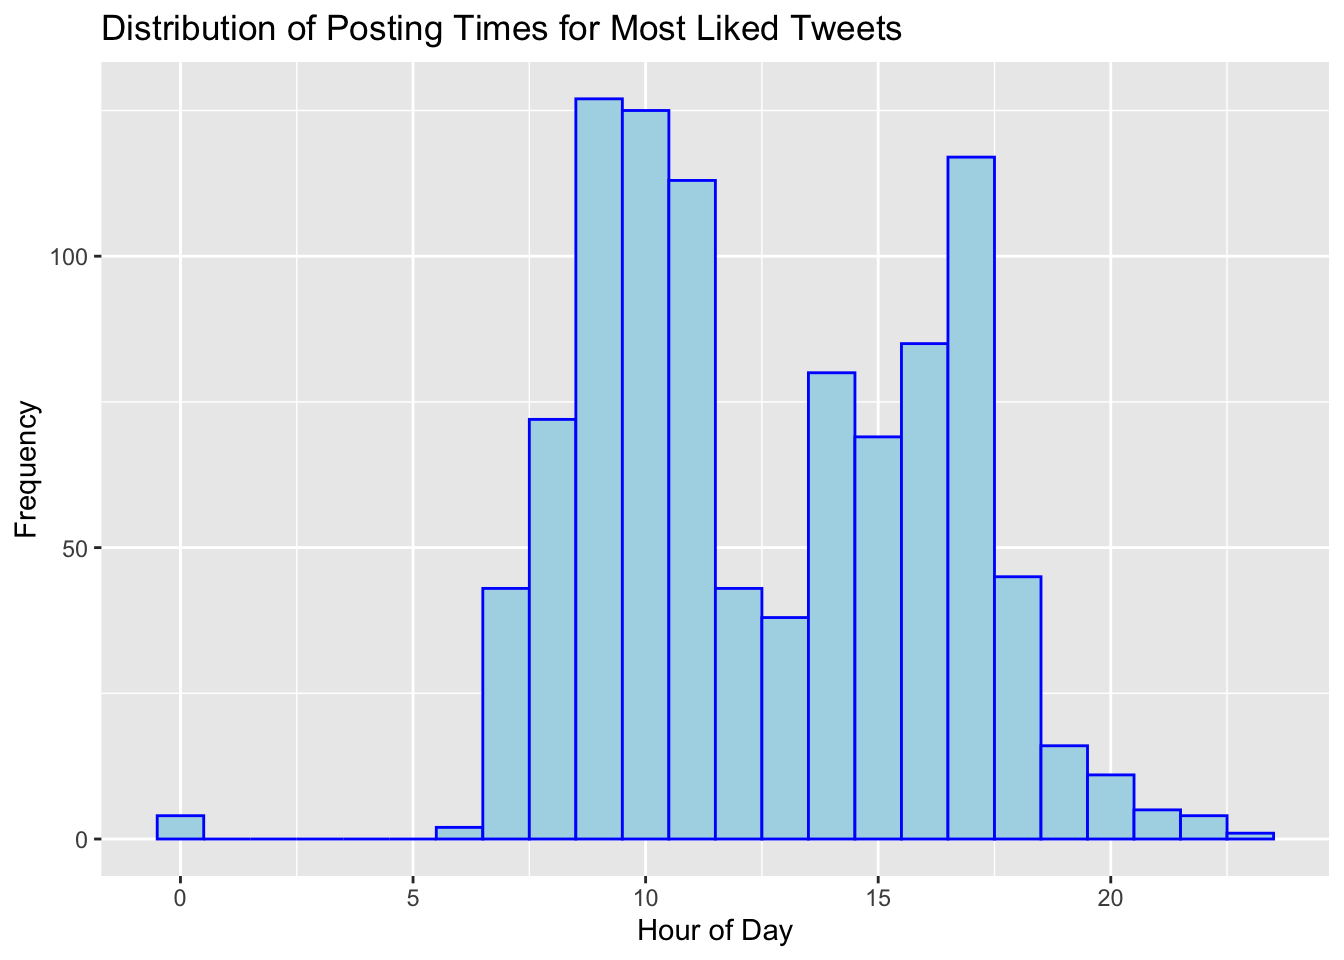
\includegraphics{Applied_Supervised_learning_Wage_prediction_Group_10_files/figure-latex/unnamed-chunk-6-1.pdf}
\#\#\# Winner Model The XGBoost model shows the best performance.
Gradient Boosting has slightly less accurate predictions based on RMSE,
MAE and R-suqred.

\begin{itemize}
\tightlist
\item
  RMSE (Root Mean Squared Error): The XGBoost Model shows an RMSE of
  26425.57.This indicates that the wage predictions are off by
  approximately CHF 26,425 from the actual salaries.
\item
  MAE (Mean Absolute Error): The MAE of 18136.72 can be interpreted as
  predictions are off by CHF 18,136 or less from the actual values.
\item
  R-squared: The R-squared of 0.662 indicates that XGBoost explains
  about 66.2\% of the variance. This means that the model captures a
  substantial portion of the factors influencing wage differences.
\end{itemize}

\subsubsection{Key Findings}\label{key-findings}

\begin{itemize}
\item
  XGBoost and Gradient Boosting (Untuned and Tuned): These models
  clearly outperform the others, with XGBoost slightly ahead in terms of
  RMSE, MAE and R-squared.
\item
  Random Forest: The tuned Random Forest model shows a noticeable
  improvement over the basic Random Forest.
\item
  Linear Regression: Is the simplest model and performs not that well,
  but is outperformed by the tree-based models (Random Forest, Gradient
  Boosting, XGBoost). \#\#\# Plot Interpretation The plot visually
  confirms the numerical results:
\item
  The XGBoost (purple) and Gradient Boosting (red/orange) points are the
  tightest around the diagonal line, signifying the best predictions.
\item
  The improvement from tuning Random Forest is evident in its slightly
  tighter clustering compared to the untuned version.
\item
  Linear Regression's points are the most scattered, reflecting its
  lower accuracy.
\end{itemize}

\subsection{Model Explanation}\label{model-explanation}

Here we aim to see which variables have the highest correlation with the
variable wage. We will use the variable importance plot to see which
variables are the most important for the model.

\begin{Shaded}
\begin{Highlighting}[]
\CommentTok{\# Variable importance for Random Forest model}
\FunctionTok{varImpPlot}\NormalTok{(rf\_model)}
\end{Highlighting}
\end{Shaded}

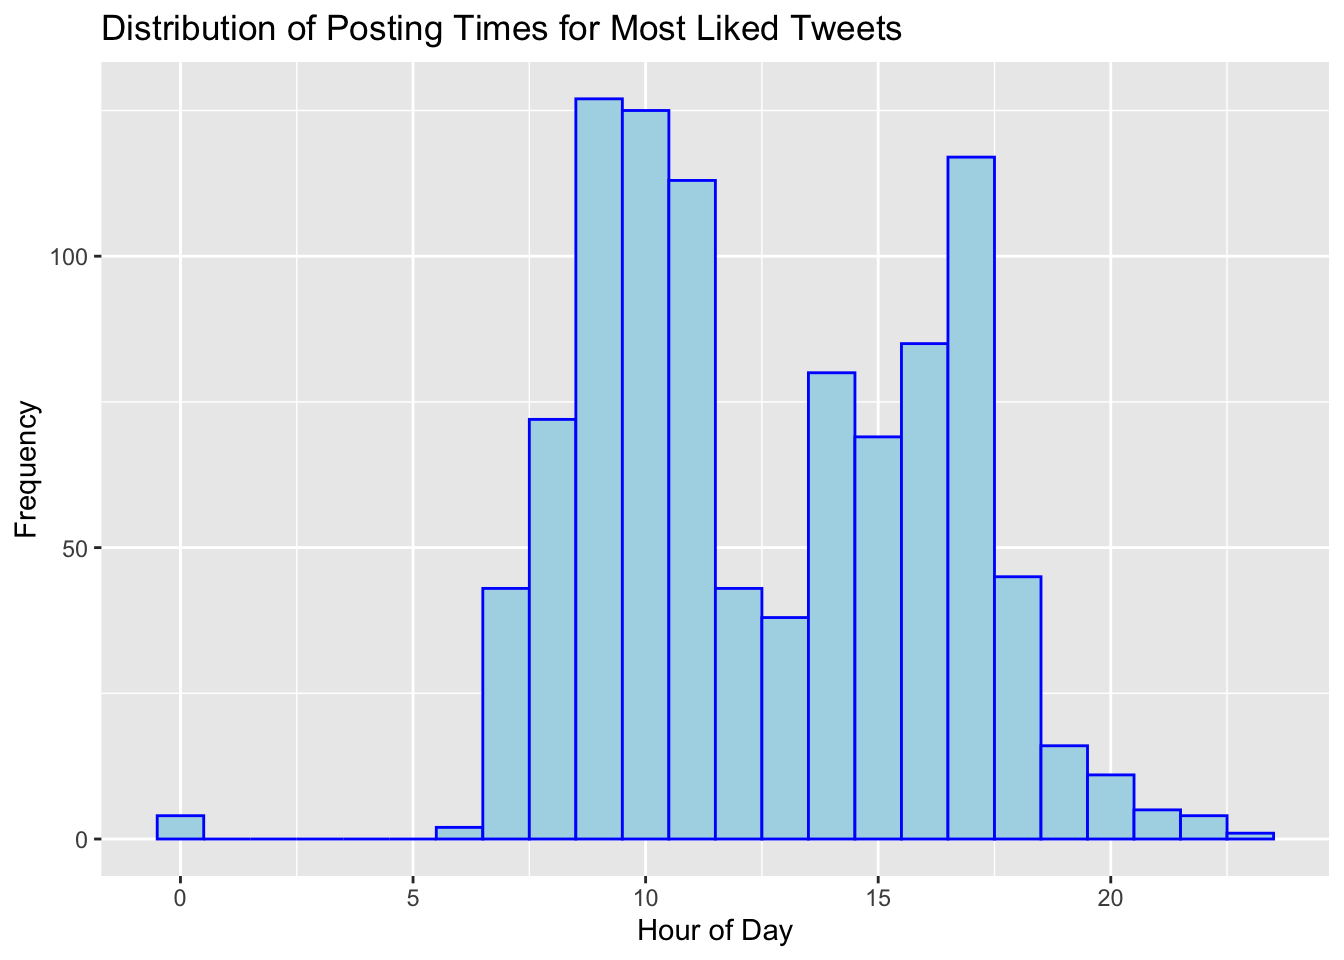
\includegraphics{Applied_Supervised_learning_Wage_prediction_Group_10_files/figure-latex/unnamed-chunk-7-1.pdf}

\begin{Shaded}
\begin{Highlighting}[]
\CommentTok{\# Summary for all models}
\ControlFlowTok{for}\NormalTok{ (model\_name }\ControlFlowTok{in} \FunctionTok{names}\NormalTok{(model\_list)) \{}
\NormalTok{  model }\OtherTok{\textless{}{-}}\NormalTok{ model\_list[[model\_name]]}
\NormalTok{  var\_imp }\OtherTok{\textless{}{-}} \FunctionTok{varImp}\NormalTok{(model)}
  \FunctionTok{cat}\NormalTok{(}\StringTok{"Variable Importance for"}\NormalTok{, model\_name, }\StringTok{"Model:}\SpecialCharTok{\textbackslash{}n}\StringTok{"}\NormalTok{)}
  \FunctionTok{print}\NormalTok{(var\_imp)}
  \FunctionTok{cat}\NormalTok{(}\StringTok{"}\SpecialCharTok{\textbackslash{}n}\StringTok{"}\NormalTok{)}
  \FunctionTok{summary}\NormalTok{(model)}
  \FunctionTok{cat}\NormalTok{(}\StringTok{"}\SpecialCharTok{\textbackslash{}n}\StringTok{"}\NormalTok{)}
\NormalTok{\}}
\end{Highlighting}
\end{Shaded}

\begin{verbatim}
## Variable Importance for Linear Regression Model:
## lm variable importance
## 
##   only 20 most important variables shown (out of 77)
## 
##                                                                                                                             Overall
## country                                                                                                                      100.00
## age                                                                                                                           99.25
## Activities_Build.prototypes.to.explore.applying.machine.learning.to.new.areas                                                 32.89
## cloud_Amazon.Web.Services..AWS.                                                                                               28.76
## ML_atwork                                                                                                                     22.77
## For.how.many.years.have.you.used.machine.learning.methods..at.work.or.in.school..                                             21.43
## Activities_Do.research.that.advances.the.state.of.the.art.of.machine.learning                                                 20.81
## experience                                                                                                                    20.26
## How.long.have.you.been.writing.code.to.analyze.data.                                                                          19.56
## industry                                                                                                                      18.22
## Programming_Bash                                                                                                              17.32
## job_role                                                                                                                      17.14
## Notebooks_Google.Colab                                                                                                        16.42
## Activities_Build.and.or.run.the.data.infrastructure.that.my.business.uses.for.storing..analyzing..and.operationalizing.data   13.99
## Activities_Analyze.and.understand.data.to.influence.product.or.business.decisions                                             13.39
## Activities_Build.and.or.run.a.machine.learning.service.that.operationally.improves.my.product.or.workflows                    13.26
## ML_framework_Spark.MLlib                                                                                                      12.93
## Programming_R                                                                                                                 12.54
## explainability.model_Examine.individual.model.coefficients                                                                    12.08
## Programming_MATLAB                                                                                                            11.40
## 
## 
## Variable Importance for Random Forest Model:
##                                                                                                                                 Overall
## gender                                                                                                                       0.23449257
## age                                                                                                                         12.60963506
## country                                                                                                                     14.73876147
## education                                                                                                                    2.44534832
## undergraduate_major                                                                                                          2.36612020
## job_role                                                                                                                    10.60376606
## industry                                                                                                                     5.09781628
## ML_atwork                                                                                                                    8.18255017
## Activities_Analyze.and.understand.data.to.influence.product.or.business.decisions                                            3.56214593
## Activities_Build.and.or.run.a.machine.learning.service.that.operationally.improves.my.product.or.workflows                   2.53655190
## Activities_Build.and.or.run.the.data.infrastructure.that.my.business.uses.for.storing..analyzing..and.operationalizing.data  3.73032192
## Activities_Build.prototypes.to.explore.applying.machine.learning.to.new.areas                                                5.82875616
## Activities_Do.research.that.advances.the.state.of.the.art.of.machine.learning                                                1.18155740
## Activities_None.of.these.activities.are.an.important.part.of.my.role.at.work                                                 2.58139191
## Notebooks_Kaggle.Kernels                                                                                                     1.60229486
## Notebooks_Google.Colab                                                                                                       2.24718987
## Notebooks_Azure.Notebook                                                                                                     3.08877179
## Notebooks_Google.Cloud.Datalab                                                                                               0.76898678
## Notebooks_JupyterHub.Binder                                                                                                  0.08368709
## Notebooks_None                                                                                                              -0.98059144
## cloud_Google.Cloud.Platform..GCP.                                                                                           -0.31107420
## cloud_Amazon.Web.Services..AWS.                                                                                              5.02486973
## cloud_Microsoft.Azure                                                                                                        0.69020350
## cloud_IBM.Cloud                                                                                                             -0.06765486
## cloud_Alibaba.Cloud                                                                                                          2.51483451
## cloud_I.have.not.used.any.cloud.providers                                                                                    4.54882226
## Programming_Python                                                                                                           2.68995962
## Programming_R                                                                                                                3.19610551
## Programming_SQL                                                                                                              3.58224790
## Programming_Bash                                                                                                             1.93759784
## Programming_Java                                                                                                             3.34319378
## Programming_Javascript.Typescript                                                                                            1.99737502
## Programming_Visual.Basic.VBA                                                                                                 1.39574484
## Programming_C.C..                                                                                                            5.02972788
## Programming_MATLAB                                                                                                           3.59073201
## Programming_Scala                                                                                                            0.50484344
## Programming_Julia                                                                                                            0.84754316
## Programming_SAS.STATA                                                                                                        1.40127958
## Programming_language_used_most_often                                                                                         4.59060049
## ML_framework_Scikit.Learn                                                                                                    1.77550204
## ML_framework_TensorFlow                                                                                                      3.05623222
## ML_framework_Keras                                                                                                           3.80976535
## ML_framework_PyTorch                                                                                                        -0.21818267
## ML_framework_Spark.MLlib                                                                                                     2.03530472
## ML_framework_H20                                                                                                             2.21896383
## ML_framework_Caret                                                                                                           2.08418169
## ML_framework_Xgboost                                                                                                         4.26980373
## ML_framework_randomForest                                                                                                   -0.30621429
## ML_framework_None                                                                                                            2.45513642
## Visualization_ggplot2                                                                                                        0.27383133
## Visualization_Matplotlib                                                                                                     2.02362674
## Visualization_Altair                                                                                                         0.17303281
## Visualization_Shiny                                                                                                          2.18301582
## Visualization_Plotly                                                                                                         0.62126763
## Visualization_None                                                                                                           1.14871955
## percent_actively.coding                                                                                                      0.69417615
## How.long.have.you.been.writing.code.to.analyze.data.                                                                         7.98292960
## For.how.many.years.have.you.used.machine.learning.methods..at.work.or.in.school..                                            7.17340080
## Do.you.consider.yourself.to.be.a.data.scientist.                                                                             1.12777852
## data_Categorical.Data                                                                                                        2.98688189
## data_Genetic.Data                                                                                                            0.37787660
## data_Geospatial.Data                                                                                                         2.94910861
## data_Image.Data                                                                                                              2.55176421
## data_Numerical.Data                                                                                                          3.49574083
## data_Sensor.Data                                                                                                             2.83774686
## data_Tabular.Data                                                                                                            2.06443228
## data_text.Data                                                                                                              -0.43494530
## data_Time.Series.Data                                                                                                        1.24578718
## data_Video.Data                                                                                                             -2.00254271
## explainability.model_Examine.individual.model.coefficients                                                                   1.20031614
## explainability.model_examine.feature.correlations                                                                            0.93143205
## explainability.model_Examine.feature.importances                                                                             3.50650402
## explainability.model_Create.partial.dependence.plots                                                                        -1.05003228
## explainability.model_LIME.functions                                                                                          1.40663039
## explainability.model_SHAP.functions                                                                                         -0.32015963
## explainability.model_None.I.do.not.use.these.model.explanation.techniques                                                    1.26479455
## experience                                                                                                                   8.76475546
## 
## 
## Variable Importance for Gradient Boosting Model:
## gbm variable importance
## 
##   only 20 most important variables shown (out of 77)
## 
##                                                                                                             Overall
## country                                                                                                    100.0000
## age                                                                                                         51.1070
## job_role                                                                                                    22.4180
## How.long.have.you.been.writing.code.to.analyze.data.                                                        13.9695
## ML_atwork                                                                                                   10.5122
## industry                                                                                                     6.7047
## cloud_Amazon.Web.Services..AWS.                                                                              5.0009
## Activities_Build.prototypes.to.explore.applying.machine.learning.to.new.areas                                3.8595
## experience                                                                                                   2.7148
## For.how.many.years.have.you.used.machine.learning.methods..at.work.or.in.school..                            2.3311
## ML_framework_Spark.MLlib                                                                                     0.8288
## education                                                                                                    0.7802
## explainability.model_Examine.feature.importances                                                             0.6130
## Programming_Bash                                                                                             0.5404
## explainability.model_LIME.functions                                                                          0.5128
## gender                                                                                                       0.5060
## Activities_Build.and.or.run.a.machine.learning.service.that.operationally.improves.my.product.or.workflows   0.4377
## ML_framework_Xgboost                                                                                         0.4323
## Programming_language_used_most_often                                                                         0.4312
## Programming_MATLAB                                                                                           0.3804
\end{verbatim}

\includegraphics{Applied_Supervised_learning_Wage_prediction_Group_10_files/figure-latex/unnamed-chunk-7-2.pdf}

\begin{verbatim}
## 
## Variable Importance for XGBoost Model:
## xgbTree variable importance
## 
##   only 20 most important variables shown (out of 77)
## 
##                                                                                                             Overall
## country                                                                                                    100.0000
## age                                                                                                         47.4221
## job_role                                                                                                    25.6616
## How.long.have.you.been.writing.code.to.analyze.data.                                                        15.0437
## ML_atwork                                                                                                    9.4756
## industry                                                                                                     8.4017
## cloud_Amazon.Web.Services..AWS.                                                                              4.4351
## Activities_Build.prototypes.to.explore.applying.machine.learning.to.new.areas                                3.3448
## experience                                                                                                   3.2768
## For.how.many.years.have.you.used.machine.learning.methods..at.work.or.in.school..                            2.1475
## ML_framework_Spark.MLlib                                                                                     1.2333
## percent_actively.coding                                                                                      0.9863
## Programming_language_used_most_often                                                                         0.9150
## education                                                                                                    0.8953
## Programming_MATLAB                                                                                           0.7018
## explainability.model_Examine.feature.importances                                                             0.6627
## Programming_Bash                                                                                             0.6040
## undergraduate_major                                                                                          0.5672
## Activities_Build.and.or.run.a.machine.learning.service.that.operationally.improves.my.product.or.workflows   0.5306
## gender                                                                                                       0.5253
## 
## 
## Variable Importance for Random Forest Tuned Model:
## rf variable importance
## 
##   only 20 most important variables shown (out of 77)
## 
##                                                                                                                             Overall
## country                                                                                                                     100.000
## age                                                                                                                          60.134
## job_role                                                                                                                     38.689
## How.long.have.you.been.writing.code.to.analyze.data.                                                                         35.811
## experience                                                                                                                   30.765
## For.how.many.years.have.you.used.machine.learning.methods..at.work.or.in.school..                                            22.977
## industry                                                                                                                     22.827
## ML_atwork                                                                                                                    21.699
## undergraduate_major                                                                                                          15.182
## cloud_Amazon.Web.Services..AWS.                                                                                              13.559
## Programming_language_used_most_often                                                                                         12.819
## Activities_Build.prototypes.to.explore.applying.machine.learning.to.new.areas                                                12.358
## Do.you.consider.yourself.to.be.a.data.scientist.                                                                             10.714
## percent_actively.coding                                                                                                      10.507
## education                                                                                                                    10.502
## Activities_Analyze.and.understand.data.to.influence.product.or.business.decisions                                             8.559
## cloud_I.have.not.used.any.cloud.providers                                                                                     6.975
## Programming_C.C..                                                                                                             6.475
## Activities_Build.and.or.run.the.data.infrastructure.that.my.business.uses.for.storing..analyzing..and.operationalizing.data   6.210
## explainability.model_Examine.feature.importances                                                                              6.199
## 
## 
## Variable Importance for Gradient Boosting Tuned Model:
## gbm variable importance
## 
##   only 20 most important variables shown (out of 77)
## 
##                                                                                                             Overall
## country                                                                                                    100.0000
## age                                                                                                         48.0833
## job_role                                                                                                    27.9569
## How.long.have.you.been.writing.code.to.analyze.data.                                                        13.9943
## ML_atwork                                                                                                   10.1426
## industry                                                                                                     8.7647
## cloud_Amazon.Web.Services..AWS.                                                                              5.0730
## experience                                                                                                   4.0096
## Activities_Build.prototypes.to.explore.applying.machine.learning.to.new.areas                                3.7164
## For.how.many.years.have.you.used.machine.learning.methods..at.work.or.in.school..                            3.4192
## education                                                                                                    1.1584
## Activities_Build.and.or.run.a.machine.learning.service.that.operationally.improves.my.product.or.workflows   1.1480
## ML_framework_Spark.MLlib                                                                                     1.1265
## Programming_language_used_most_often                                                                         1.0519
## percent_actively.coding                                                                                      1.0473
## undergraduate_major                                                                                          0.8708
## ML_framework_Xgboost                                                                                         0.6861
## gender                                                                                                       0.6557
## Activities_Do.research.that.advances.the.state.of.the.art.of.machine.learning                                0.5768
## Programming_Bash                                                                                             0.5715
\end{verbatim}

\includegraphics{Applied_Supervised_learning_Wage_prediction_Group_10_files/figure-latex/unnamed-chunk-7-3.pdf}

\subsubsection{Insights from Model Comparison
(General):}\label{insights-from-model-comparison-general}

Several factors continue to show a strong explainability of wages across
all models:

\begin{itemize}
\tightlist
\item
  Country: The country is a major factor when wages are predicted. This
  is likely because the variations in cost of living, industry
  concentration, and demand for machine learning talent. Then when a
  country has more machine learning jobs, this rises the explainability
  for the wage related to machine learning usage at work. (See below)
\item
  Age and Experience: Age and years of experience are consistently
  strong predictors. This suggests that wages generally increase with
  maturity and expertise.
\item
  Job Role: The job role has impacts on the wage. This is likely because
  different roles require different skill sets and responsibilities.
\item
  Coding Experience for Data Analysis: The length of time spent coding
  continues to emerge as a impactful factor. This may also be connected
  with age and experience.
\item
  Machine Learning Usage at Work (ML\_atwork): Whether or not someone
  utilizes machine learning in their work is a consistent predictor.
  This may also be connected with the job role and country.
\item
  Cloud Experience (AWS): Experience with Amazon Web Services (AWS)
  stands out as a factor in several models. This can reflect the
  widespread adoption of AWS in the industry.
\item
  Domain-Specific Factors: Various domain-specific variables, such as
  machine learning activities or framework usage. \#\#\# Model-Specific
  Insights \#\#\#\# Linear Regression: The linear regression model
  emphasizes country, age, and experience, aligning with the expectation
  of linear relationships between these factors and salary. AWS
  experience is notably prominent, suggesting a potential salary premium
  for professionals with this skill. \#\#\#\# Random Forest: Compared to
  linear regression, the random forest model distributes importance more
  evenly across various predictors. Country, age, job role, and
  experience remain significant factors. Notably, specific programming
  languages and tools gain importance, indicating that tool preferences
  might influence salary in complex, non-linear ways. \#\#\#\# Gradient
  Boosting: The gradient boosting model shows a stronger focus on
  country, age, and job role. Time spent coding for data analysis
  emerges as a top predictor, reinforcing the value of practical coding
  skills in this domain. \#\#\#\# XGBoost: The XGBoost model closely
  aligns with the gradient boosting model in terms of variable
  importance, with country, age, coding experience, and job role. This
  alignment between the two top-performing models provides strong
  evidence for the relevance of these factors in determining salary.
  \#\#\#\# Tuned Models (Random Forest and Gradient Boosting): The tuned
  models show similar variable importance as their untuned models, with
  minor shifts in rankings. This suggests that the overall relationships
  between predictors and salary remain stable.
\end{itemize}

\subsection{Wage Prediction:}\label{wage-prediction}

\begin{Shaded}
\begin{Highlighting}[]
\CommentTok{\# Load and prepare the team data}
\FunctionTok{set.seed}\NormalTok{(}\DecValTok{123}\NormalTok{)}
\NormalTok{team\_data }\OtherTok{\textless{}{-}} \FunctionTok{read\_csv}\NormalTok{(}\StringTok{"./team\_data.csv"}\NormalTok{)}

\CommentTok{\# Add experience column with consistent levels}
\NormalTok{team\_data}\SpecialCharTok{$}\NormalTok{experience }\OtherTok{\textless{}{-}} \FunctionTok{factor}\NormalTok{(}
\NormalTok{  team\_data}\SpecialCharTok{$}\NormalTok{years\_experience,}
  \AttributeTok{levels =} \FunctionTok{c}\NormalTok{(}
    \StringTok{"0{-}1"}\NormalTok{, }\StringTok{"1{-}2"}\NormalTok{, }\StringTok{"2{-}3"}\NormalTok{, }\StringTok{"3{-}4"}\NormalTok{, }\StringTok{"4{-}5"}\NormalTok{, }\StringTok{"5{-}11"}\NormalTok{,}
    \StringTok{"11{-}15"}\NormalTok{, }\StringTok{"15{-}20"}\NormalTok{, }\StringTok{"20{-}25"}\NormalTok{, }\StringTok{"25{-}30"}\NormalTok{, }\StringTok{"30 +"}
\NormalTok{  ),}
  \AttributeTok{ordered =} \ConstantTok{TRUE}
\NormalTok{)}
\CommentTok{\# Remove years\_experience column and first column}
\NormalTok{team\_data }\OtherTok{\textless{}{-}}\NormalTok{ team\_data[, }\SpecialCharTok{{-}}\DecValTok{1}\NormalTok{] }\SpecialCharTok{\%\textgreater{}\%} \FunctionTok{select}\NormalTok{(}\SpecialCharTok{{-}}\NormalTok{years\_experience)}
\CommentTok{\# Ensure factor levels in team\_data match those in data\_wage}
\ControlFlowTok{for}\NormalTok{ (col }\ControlFlowTok{in} \FunctionTok{names}\NormalTok{(team\_data)) \{}
  \ControlFlowTok{if}\NormalTok{ (}\FunctionTok{is.character}\NormalTok{(team\_data[[col]])) \{}
\NormalTok{    levels\_in\_wage\_data }\OtherTok{\textless{}{-}} \FunctionTok{levels}\NormalTok{(data\_wage[[col]])}
\NormalTok{    team\_data[[col]] }\OtherTok{\textless{}{-}} \FunctionTok{factor}\NormalTok{(team\_data[[col]], }\AttributeTok{levels =}\NormalTok{ levels\_in\_wage\_data)}
\NormalTok{  \}}
\NormalTok{\}}
\CommentTok{\# One{-}hot encode categorical variables and scale numeric variables}
\NormalTok{team\_data\_encoded }\OtherTok{\textless{}{-}}\NormalTok{ team\_data }\SpecialCharTok{\%\textgreater{}\%}
  \FunctionTok{mutate}\NormalTok{(}\FunctionTok{across}\NormalTok{(}
    \FunctionTok{where}\NormalTok{(is.character),}
    \SpecialCharTok{\textasciitilde{}} \FunctionTok{factor}\NormalTok{(.x, }\AttributeTok{levels =} \FunctionTok{levels}\NormalTok{(data\_wage[[}\FunctionTok{cur\_column}\NormalTok{()]]))}
\NormalTok{  )) }\SpecialCharTok{\%\textgreater{}\%}
  \FunctionTok{mutate}\NormalTok{(}\FunctionTok{across}\NormalTok{(}\FunctionTok{where}\NormalTok{(is.numeric), }\SpecialCharTok{\textasciitilde{}} \FunctionTok{scale}\NormalTok{(.x))) }\SpecialCharTok{\%\textgreater{}\%}
  \FunctionTok{mutate}\NormalTok{(}\FunctionTok{across}\NormalTok{(}\FunctionTok{where}\NormalTok{(is.factor), }\SpecialCharTok{\textasciitilde{}} \FunctionTok{as.numeric}\NormalTok{(}\FunctionTok{as.factor}\NormalTok{(.x)) }\SpecialCharTok{{-}} \DecValTok{1}\NormalTok{))}
\CommentTok{\# Apply dummy variable encoding}
\NormalTok{team\_data\_transformed }\OtherTok{\textless{}{-}} \FunctionTok{as.data.frame}\NormalTok{(}
  \FunctionTok{predict}\NormalTok{(dummies, }\AttributeTok{newdata =}\NormalTok{ team\_data\_encoded)}
\NormalTok{)}
\CommentTok{\# Use XGBoost model for prediction}
\NormalTok{pred\_xgboost }\OtherTok{\textless{}{-}} \FunctionTok{predict}\NormalTok{(xgboost\_model, }\AttributeTok{newdata =}\NormalTok{ team\_data\_transformed)}
\FunctionTok{print}\NormalTok{(pred\_xgboost)}
\end{Highlighting}
\end{Shaded}

\begin{verbatim}
## [1] 43798.56 33963.88 41666.16 37151.39
\end{verbatim}

\begin{Shaded}
\begin{Highlighting}[]
\CommentTok{\# Replace NAs with 0 in team\_data}
\NormalTok{team\_data\_transformed[}\FunctionTok{is.na}\NormalTok{(team\_data\_transformed)] }\OtherTok{\textless{}{-}} \DecValTok{0}
\CommentTok{\# use gbm\_model for prediction}
\NormalTok{pred\_gbm }\OtherTok{\textless{}{-}} \FunctionTok{predict}\NormalTok{(gbm\_tuned, }\AttributeTok{newdata =}\NormalTok{ team\_data\_transformed)}
\FunctionTok{print}\NormalTok{(pred\_gbm)}
\end{Highlighting}
\end{Shaded}

\begin{verbatim}
## [1] 40183.47 26912.31 24531.97 36606.36
\end{verbatim}

Until the end we could not factor the data\_wage properties to our
custom team data set which is why we could not predict the wages for the
team members exactly. For example the prediction with the gbm\_model
does not work because of the NA values in the team\_data. We would have
to replace the NA values with 0 in order to make the prediction work.
This would distort the prediction. We will stick to the XGBoost model
for our predictions and ignore the wages of gbm tuned model.

\subsubsection{Interpreting the
Predictions:}\label{interpreting-the-predictions}

XGBoost predicts wages of 43798.56 33963.88 41666.16 and 37151.39 for
the four team members. All of the team do have a higher yearly wage.
This shows that eather the team members are not well displayed in the
team data set or the MAE of 18136.72 has a big impact on the wage. The
predictions are based on the model's learned relationships between the
variables like country and experience and wages. The predictions provide
an estimate of the expected salary for each team member based on these
factors. When a team member has more years of experience this than noted
in the dataset this could lead to a higher wage than now printed.

\subsubsection{Impact of Replacing NAs with
0:}\label{impact-of-replacing-nas-with-0}

Replacing missing values (NAs) with zeros will propably distort the
predictions:

\begin{itemize}
\tightlist
\item
  Meaning Change: Zeros has a specific meaning in data (e.g., absence of
  a characteristic). Replacing NAs with zeros has changed the
  interpretation of the data.
\item
  Skewed Relationships: Zeros skew the relationships between variables.
  If a model learned a relationship based on actual zeros, it make
  incorrect assumptions.
\item
  Loss of Information: Replacing NAs with zeros discards information.
\end{itemize}

\subsection{H2O AutoML analysis}\label{h2o-automl-analysis}

\begin{Shaded}
\begin{Highlighting}[]
\CommentTok{\# H2O AutoML Setup}
\FunctionTok{h2o.init}\NormalTok{()}
\end{Highlighting}
\end{Shaded}

\begin{verbatim}
##  Connection successful!
## 
## R is connected to the H2O cluster: 
##     H2O cluster uptime:         1 days 23 hours 
##     H2O cluster timezone:       Europe/Zurich 
##     H2O data parsing timezone:  UTC 
##     H2O cluster version:        3.44.0.3 
##     H2O cluster version age:    5 months and 6 days 
##     H2O cluster name:           H2O_started_from_R_mischahaenen_xvp655 
##     H2O cluster total nodes:    1 
##     H2O cluster total memory:   7.08 GB 
##     H2O cluster total cores:    10 
##     H2O cluster allowed cores:  10 
##     H2O cluster healthy:        TRUE 
##     H2O Connection ip:          localhost 
##     H2O Connection port:        54321 
##     H2O Connection proxy:       NA 
##     H2O Internal Security:      FALSE 
##     R Version:                  R version 4.4.0 (2024-04-24)
\end{verbatim}

\begin{Shaded}
\begin{Highlighting}[]
\CommentTok{\# Convert the dataset to H2O object}
\NormalTok{h2o\_data }\OtherTok{\textless{}{-}} \FunctionTok{as.h2o}\NormalTok{(data\_transformed)}
\end{Highlighting}
\end{Shaded}

\begin{verbatim}
##   |                                                                              |                                                                      |   0%  |                                                                              |======================================================================| 100%
\end{verbatim}

\begin{Shaded}
\begin{Highlighting}[]
\CommentTok{\# Split dataset into training and validation sets}
\NormalTok{splits }\OtherTok{\textless{}{-}} \FunctionTok{h2o.splitFrame}\NormalTok{(h2o\_data, }\AttributeTok{ratios =} \FunctionTok{c}\NormalTok{(}\FloatTok{0.8}\NormalTok{), }\AttributeTok{seed =} \DecValTok{12}\NormalTok{)}
\NormalTok{train }\OtherTok{\textless{}{-}}\NormalTok{ splits[[}\DecValTok{1}\NormalTok{]]}
\NormalTok{valid }\OtherTok{\textless{}{-}}\NormalTok{ splits[[}\DecValTok{2}\NormalTok{]]}

\CommentTok{\# Set the dependent variable}
\NormalTok{dep\_var }\OtherTok{\textless{}{-}} \StringTok{"wage"}

\CommentTok{\# Run H2O AutoML}
\NormalTok{automl }\OtherTok{\textless{}{-}} \FunctionTok{h2o.automl}\NormalTok{(}
  \AttributeTok{x =} \FunctionTok{setdiff}\NormalTok{(}\FunctionTok{colnames}\NormalTok{(h2o\_data), dep\_var),}
  \AttributeTok{y =}\NormalTok{ dep\_var,}
  \AttributeTok{training\_frame =}\NormalTok{ train,}
  \AttributeTok{max\_runtime\_secs =} \DecValTok{600}\NormalTok{,}
  \AttributeTok{seed =} \DecValTok{12}
\NormalTok{)}
\end{Highlighting}
\end{Shaded}

\begin{verbatim}
##   |                                                                              |                                                                      |   0%  |                                                                              |==                                                                    |   2%
## 14:26:25.160: AutoML: XGBoost is not available; skipping it.  |                                                                              |==                                                                    |   3%  |                                                                              |====                                                                  |   6%  |                                                                              |=====                                                                 |   7%  |                                                                              |=====                                                                 |   8%  |                                                                              |======                                                                |   8%  |                                                                              |======                                                                |   9%  |                                                                              |=======                                                               |  10%  |                                                                              |========                                                              |  12%  |                                                                              |=========                                                             |  13%  |                                                                              |==========                                                            |  14%  |                                                                              |=============                                                         |  18%  |                                                                              |=============                                                         |  19%  |                                                                              |==============                                                        |  19%  |                                                                              |==============                                                        |  20%  |                                                                              |===============                                                       |  22%  |                                                                              |================                                                      |  23%  |                                                                              |====================                                                  |  28%  |                                                                              |====================                                                  |  29%  |                                                                              |=====================                                                 |  29%  |                                                                              |=====================                                                 |  30%  |                                                                              |=====================                                                 |  31%  |                                                                              |======================                                                |  31%  |                                                                              |======================                                                |  32%  |                                                                              |=======================                                               |  32%  |                                                                              |=======================                                               |  33%  |                                                                              |========================                                              |  34%  |                                                                              |========================                                              |  35%  |                                                                              |=========================                                             |  35%  |                                                                              |=========================                                             |  36%  |                                                                              |==========================                                            |  37%  |                                                                              |==========================                                            |  38%  |                                                                              |===========================                                           |  38%  |                                                                              |===========================                                           |  39%  |                                                                              |============================                                          |  39%  |                                                                              |============================                                          |  40%  |                                                                              |=============================                                         |  41%  |                                                                              |=============================                                         |  42%  |                                                                              |==============================                                        |  42%  |                                                                              |==============================                                        |  43%  |                                                                              |===============================                                       |  44%  |                                                                              |===============================                                       |  45%  |                                                                              |================================                                      |  45%  |                                                                              |================================                                      |  46%  |                                                                              |=================================                                     |  47%  |                                                                              |=================================                                     |  48%  |                                                                              |==================================                                    |  48%  |                                                                              |==================================                                    |  49%  |                                                                              |===================================                                   |  50%  |                                                                              |===================================                                   |  51%  |                                                                              |====================================                                  |  51%  |                                                                              |====================================                                  |  52%  |                                                                              |=====================================                                 |  52%  |                                                                              |=====================================                                 |  53%  |                                                                              |======================================                                |  54%  |                                                                              |======================================                                |  55%  |                                                                              |=======================================                               |  55%  |                                                                              |=======================================                               |  56%  |                                                                              |========================================                              |  57%  |                                                                              |========================================                              |  58%  |                                                                              |=========================================                             |  58%  |                                                                              |=========================================                             |  59%  |                                                                              |==========================================                            |  59%  |                                                                              |==========================================                            |  60%  |                                                                              |===========================================                           |  61%  |                                                                              |===========================================                           |  62%  |                                                                              |============================================                          |  62%  |                                                                              |============================================                          |  63%  |                                                                              |=============================================                         |  64%  |                                                                              |=============================================                         |  65%  |                                                                              |==============================================                        |  65%  |                                                                              |==============================================                        |  66%  |                                                                              |===============================================                       |  67%  |                                                                              |===============================================                       |  68%  |                                                                              |================================================                      |  68%  |                                                                              |================================================                      |  69%  |                                                                              |=================================================                     |  69%  |                                                                              |=================================================                     |  70%  |                                                                              |=================================================                     |  71%  |                                                                              |==================================================                    |  71%  |                                                                              |==================================================                    |  72%  |                                                                              |===================================================                   |  72%  |                                                                              |===================================================                   |  73%  |                                                                              |====================================================                  |  74%  |                                                                              |====================================================                  |  75%  |                                                                              |=====================================================                 |  75%  |                                                                              |=====================================================                 |  76%  |                                                                              |======================================================                |  77%  |                                                                              |======================================================                |  78%  |                                                                              |=======================================================               |  78%  |                                                                              |======================================================================| 100%
\end{verbatim}

\begin{Shaded}
\begin{Highlighting}[]
\CommentTok{\# View leaderboard of models generated by AutoML}
\NormalTok{lb }\OtherTok{\textless{}{-}}\NormalTok{ automl}\SpecialCharTok{@}\NormalTok{leaderboard}
\FunctionTok{print}\NormalTok{(lb, }\AttributeTok{n =} \FunctionTok{nrow}\NormalTok{(lb))}
\end{Highlighting}
\end{Shaded}

\begin{verbatim}
##                                                   model_id     rmse        mse
## 1     StackedEnsemble_AllModels_2_AutoML_4_20240527_142625 26139.05  683250139
## 2     StackedEnsemble_AllModels_1_AutoML_4_20240527_142625 26195.51  686204784
## 3  StackedEnsemble_BestOfFamily_2_AutoML_4_20240527_142625 26446.63  699424260
## 4  StackedEnsemble_BestOfFamily_3_AutoML_4_20240527_142625 26447.76  699483967
## 5                           GBM_2_AutoML_4_20240527_142625 26448.68  699532927
## 6             GBM_grid_1_AutoML_4_20240527_142625_model_50 26497.95  702141257
## 7             GBM_grid_1_AutoML_4_20240527_142625_model_40 26528.26  703748767
## 8                           GBM_3_AutoML_4_20240527_142625 26566.21  705763394
## 9                           GBM_5_AutoML_4_20240527_142625 26635.24  709435912
## 10             GBM_grid_1_AutoML_4_20240527_142625_model_2 26635.95  709473949
## 11            GBM_grid_1_AutoML_4_20240527_142625_model_11 26646.82  710052994
## 12            GBM_grid_1_AutoML_4_20240527_142625_model_16 26681.86  711921630
## 13            GBM_grid_1_AutoML_4_20240527_142625_model_54 26718.94  713901497
## 14             GBM_grid_1_AutoML_4_20240527_142625_model_1 26751.83  715660668
## 15            GBM_grid_1_AutoML_4_20240527_142625_model_13 26759.06  716047534
## 16            GBM_grid_1_AutoML_4_20240527_142625_model_17 26792.13  717818438
## 17            GBM_grid_1_AutoML_4_20240527_142625_model_14 26902.42  723740463
## 18             GBM_grid_1_AutoML_4_20240527_142625_model_4 26919.73  724671816
## 19            GBM_grid_1_AutoML_4_20240527_142625_model_24 26932.79  725375355
## 20             GBM_grid_1_AutoML_4_20240527_142625_model_5 26949.65  726283374
## 21             GBM_grid_1_AutoML_4_20240527_142625_model_7 26968.33  727290906
## 22            GBM_grid_1_AutoML_4_20240527_142625_model_47 26988.98  728404784
## 23                          GBM_4_AutoML_4_20240527_142625 27009.60  729518345
## 24            GBM_grid_1_AutoML_4_20240527_142625_model_20 27014.63  729790321
## 25             GBM_grid_1_AutoML_4_20240527_142625_model_8 27030.65  730656091
## 26             GBM_grid_1_AutoML_4_20240527_142625_model_6 27034.54  730866390
## 27            GBM_grid_1_AutoML_4_20240527_142625_model_27 27053.88  731912276
## 28            GBM_grid_1_AutoML_4_20240527_142625_model_32 27124.78  735753561
## 29            GBM_grid_1_AutoML_4_20240527_142625_model_22 27158.92  737606821
## 30            GBM_grid_1_AutoML_4_20240527_142625_model_44 27169.71  738193196
## 31            GBM_grid_1_AutoML_4_20240527_142625_model_15 27174.21  738437958
## 32            GBM_grid_1_AutoML_4_20240527_142625_model_46 27174.81  738470490
## 33            GBM_grid_1_AutoML_4_20240527_142625_model_48 27214.09  740606756
## 34            GBM_grid_1_AutoML_4_20240527_142625_model_59 27292.72  744892559
## 35            GBM_grid_1_AutoML_4_20240527_142625_model_35 27293.08  744912337
## 36            GBM_grid_1_AutoML_4_20240527_142625_model_58 27370.61  749150187
## 37            GBM_grid_1_AutoML_4_20240527_142625_model_41 27427.25  752254146
## 38            GBM_grid_1_AutoML_4_20240527_142625_model_30 27439.71  752937714
## 39            GBM_grid_1_AutoML_4_20240527_142625_model_60 27445.99  753282238
## 40 StackedEnsemble_BestOfFamily_1_AutoML_4_20240527_142625 27457.01  753887163
## 41                          GBM_1_AutoML_4_20240527_142625 27462.28  754176930
## 42            GBM_grid_1_AutoML_4_20240527_142625_model_45 27562.45  759688440
## 43            GBM_grid_1_AutoML_4_20240527_142625_model_49 27637.57  763835546
## 44            GBM_grid_1_AutoML_4_20240527_142625_model_10 27689.98  766735112
## 45            GBM_grid_1_AutoML_4_20240527_142625_model_34 27691.52  766820173
## 46            GBM_grid_1_AutoML_4_20240527_142625_model_19 27741.70  769601888
## 47            GBM_grid_1_AutoML_4_20240527_142625_model_25 27747.85  769943440
## 48            GBM_grid_1_AutoML_4_20240527_142625_model_26 27784.49  771977922
## 49            GBM_grid_1_AutoML_4_20240527_142625_model_55 27796.10  772623419
## 50            GBM_grid_1_AutoML_4_20240527_142625_model_39 27817.75  773827255
## 51            GBM_grid_1_AutoML_4_20240527_142625_model_53 27849.59  775599523
## 52            GBM_grid_1_AutoML_4_20240527_142625_model_21 27890.82  777897636
## 53             GBM_grid_1_AutoML_4_20240527_142625_model_3 27965.43  782065355
## 54            GBM_grid_1_AutoML_4_20240527_142625_model_57 27991.85  783543534
## 55            GBM_grid_1_AutoML_4_20240527_142625_model_56 27993.50  783636165
## 56            GBM_grid_1_AutoML_4_20240527_142625_model_51 27998.46  783913585
## 57            GBM_grid_1_AutoML_4_20240527_142625_model_52 28006.42  784359360
## 58            GBM_grid_1_AutoML_4_20240527_142625_model_33 28011.82  784661916
## 59            GBM_grid_1_AutoML_4_20240527_142625_model_37 28023.60  785322313
## 60            GBM_grid_1_AutoML_4_20240527_142625_model_36 28046.19  786588773
## 61            GBM_grid_1_AutoML_4_20240527_142625_model_43 28087.27  788894991
## 62            GBM_grid_1_AutoML_4_20240527_142625_model_38 28092.83  789207081
## 63            GBM_grid_1_AutoML_4_20240527_142625_model_42 28200.00  795239923
## 64            GBM_grid_1_AutoML_4_20240527_142625_model_61 28227.53  796793537
## 65            GBM_grid_1_AutoML_4_20240527_142625_model_28 28445.69  809157537
## 66            GBM_grid_1_AutoML_4_20240527_142625_model_23 28512.45  812959636
## 67            GBM_grid_1_AutoML_4_20240527_142625_model_31 28700.12  823696854
## 68             GBM_grid_1_AutoML_4_20240527_142625_model_9 28994.69  840691787
## 69            GBM_grid_1_AutoML_4_20240527_142625_model_29 29053.92  844130394
## 70                          DRF_1_AutoML_4_20240527_142625 29056.03  844252867
## 71            GBM_grid_1_AutoML_4_20240527_142625_model_18 29106.19  847170440
## 72                          XRT_1_AutoML_4_20240527_142625 29280.58  857352545
## 73            GBM_grid_1_AutoML_4_20240527_142625_model_12 29385.90  863531133
## 74                 DeepLearning_1_AutoML_4_20240527_142625 34644.59 1200247790
## 75            GBM_grid_1_AutoML_4_20240527_142625_model_62 34653.42 1200859414
## 76                          GLM_1_AutoML_4_20240527_142625 45471.23 2067632637
##         mae    rmsle mean_residual_deviance
## 1  18107.75      NaN              683250139
## 2  18135.04      NaN              686204784
## 3  18376.06      NaN              699424260
## 4  18375.23      NaN              699483967
## 5  18424.63      NaN              699532927
## 6  18430.52      NaN              702141257
## 7  18568.50      NaN              703748767
## 8  18516.35      NaN              705763394
## 9  18638.08      NaN              709435912
## 10 18566.23      NaN              709473949
## 11 18595.78      NaN              710052994
## 12 18879.91      NaN              711921630
## 13 18758.09      NaN              713901497
## 14 18893.10      NaN              715660668
## 15 18759.59      NaN              716047534
## 16 18816.02      NaN              717818438
## 17 19017.39      NaN              723740463
## 18 18955.03      NaN              724671816
## 19 18828.14      NaN              725375355
## 20 18879.64      NaN              726283374
## 21 18958.86      NaN              727290906
## 22 19043.54      NaN              728404784
## 23 18917.85      NaN              729518345
## 24 19184.56      NaN              729790321
## 25 18840.89      NaN              730656091
## 26 18972.96      NaN              730866390
## 27 19124.66      NaN              731912276
## 28 18982.02      NaN              735753561
## 29 19320.22      NaN              737606821
## 30 19061.13      NaN              738193196
## 31 19362.26      NaN              738437958
## 32 19052.18      NaN              738470490
## 33 19216.95      NaN              740606756
## 34 19088.58      NaN              744892559
## 35 19347.58      NaN              744912337
## 36 19318.84      NaN              749150187
## 37 19486.72      NaN              752254146
## 38 19134.98      NaN              752937714
## 39 19335.40      NaN              753282238
## 40 19153.68      NaN              753887163
## 41 19183.27      NaN              754176930
## 42 19321.66      NaN              759688440
## 43 19681.10      NaN              763835546
## 44 19439.10      NaN              766735112
## 45 19345.92      NaN              766820173
## 46 19611.89      NaN              769601888
## 47 19722.01      NaN              769943440
## 48 19681.69      NaN              771977922
## 49 19580.60      NaN              772623419
## 50 19692.38      NaN              773827255
## 51 19549.62      NaN              775599523
## 52 19993.74      NaN              777897636
## 53 19762.75      NaN              782065355
## 54 19840.18      NaN              783543534
## 55 19697.51      NaN              783636165
## 56 19745.15      NaN              783913585
## 57 19823.26      NaN              784359360
## 58 20111.61      NaN              784661916
## 59 19730.67      NaN              785322313
## 60 19991.29      NaN              786588773
## 61 19894.31      NaN              788894991
## 62 19835.08      NaN              789207081
## 63 20278.18      NaN              795239923
## 64 19984.40      NaN              796793537
## 65 20625.04      NaN              809157537
## 66 20497.91      NaN              812959636
## 67 20481.36      NaN              823696854
## 68 20651.17 2.998277              840691787
## 69 20767.06      NaN              844130394
## 70 20922.92 3.029713              844252867
## 71 21239.19      NaN              847170440
## 72 21311.85 3.054159              857352545
## 73 21413.42 3.042164              863531133
## 74 25629.15      NaN             1200247790
## 75 27368.01 3.320113             1200859414
## 76 36843.21 3.486076             2067632637
## 
## [76 rows x 6 columns]
\end{verbatim}

\begin{Shaded}
\begin{Highlighting}[]
\CommentTok{\# Export leaderboard to Excel}
\NormalTok{lb\_table }\OtherTok{\textless{}{-}} \FunctionTok{as.data.table}\NormalTok{(lb)}
\FunctionTok{write\_xlsx}\NormalTok{(lb\_table, }\StringTok{"./trained\_ML\_models.xlsx"}\NormalTok{)}

\CommentTok{\# Find the best performing model per a certain criterion and explore it}
\NormalTok{best\_model }\OtherTok{\textless{}{-}} \FunctionTok{h2o.get\_best\_model}\NormalTok{(automl, }\AttributeTok{criterion =} \StringTok{"rmse"}\NormalTok{)}
\NormalTok{best\_model}
\end{Highlighting}
\end{Shaded}

\begin{verbatim}
## Model Details:
## ==============
## 
## H2ORegressionModel: stackedensemble
## Model ID:  StackedEnsemble_AllModels_2_AutoML_4_20240527_142625 
## Model Summary for Stacked Ensemble: 
##                                          key            value
## 1                          Stacking strategy cross_validation
## 2       Number of base models (used / total)              4/9
## 3           # GBM base models (used / total)              4/5
## 4           # DRF base models (used / total)              0/2
## 5  # DeepLearning base models (used / total)              0/1
## 6           # GLM base models (used / total)              0/1
## 7                      Metalearner algorithm              GLM
## 8         Metalearner fold assignment scheme           Random
## 9                         Metalearner nfolds                5
## 10                   Metalearner fold_column               NA
## 11        Custom metalearner hyperparameters             None
## 
## 
## H2ORegressionMetrics: stackedensemble
## ** Reported on training data. **
## 
## MSE:  304595752
## RMSE:  17452.67
## MAE:  12187.37
## RMSLE:  NaN
## Mean Residual Deviance :  304595752
## 
## 
## 
## H2ORegressionMetrics: stackedensemble
## ** Reported on cross-validation data. **
## ** 5-fold cross-validation on training data (Metrics computed for combined holdout predictions) **
## 
## MSE:  683250139
## RMSE:  26139.05
## MAE:  18107.75
## RMSLE:  NaN
## Mean Residual Deviance :  683250139
## 
## 
## Cross-Validation Metrics Summary: 
##                                        mean                  sd
## mae                            18107.229000          204.924320
## mean_residual_deviance     683025900.000000     22266594.000000
## mse                        683025900.000000     22266594.000000
## null_deviance          3496712000000.000000 150906000000.000000
## r2                                 0.669528            0.011805
## residual_deviance      1155512700000.000000  69518040000.000000
## rmse                           26131.986000          426.038970
## rmsle                                    NA            0.000000
##                                  cv_1_valid           cv_2_valid
## mae                            18098.504000         18362.922000
## mean_residual_deviance     691395500.000000     687286140.000000
## mse                        691395500.000000     687286140.000000
## null_deviance          3530045800000.000000 3491709600000.000000
## r2                                 0.656026             0.665650
## residual_deviance      1214090600000.000000 1167011900000.000000
## rmse                           26294.400000         26216.143000
## rmsle                                    NA                   NA
##                                  cv_3_valid           cv_4_valid
## mae                            18226.734000         17821.310000
## mean_residual_deviance     712753300.000000     654290200.000000
## mse                        712753300.000000     654290200.000000
## null_deviance          3624694200000.000000 3593710000000.000000
## r2                                 0.663635             0.686390
## residual_deviance      1218808100000.000000 1126687700000.000000
## rmse                           26697.440000         25579.098000
## rmsle                                    NA                   NA
##                                  cv_5_valid
## mae                            18026.668000
## mean_residual_deviance     669404400.000000
## mse                        669404400.000000
## null_deviance          3243401300000.000000
## r2                                 0.675937
## residual_deviance      1050964900000.000000
## rmse                           25872.850000
## rmsle                                    NA
\end{verbatim}

\begin{Shaded}
\begin{Highlighting}[]
\CommentTok{\# Predictions and performance on the validation set}
\NormalTok{pred\_best\_model }\OtherTok{\textless{}{-}} \FunctionTok{h2o.predict}\NormalTok{(best\_model, valid)}
\end{Highlighting}
\end{Shaded}

\begin{verbatim}
##   |                                                                              |                                                                      |   0%  |                                                                              |======================================================================| 100%
\end{verbatim}

\begin{Shaded}
\begin{Highlighting}[]
\NormalTok{perf\_best\_model }\OtherTok{\textless{}{-}} \FunctionTok{h2o.performance}\NormalTok{(best\_model, valid)}

\CommentTok{\# Summarize the performance}
\NormalTok{rmse }\OtherTok{\textless{}{-}} \FunctionTok{h2o.rmse}\NormalTok{(perf\_best\_model)}
\NormalTok{mae }\OtherTok{\textless{}{-}} \FunctionTok{h2o.mae}\NormalTok{(perf\_best\_model)}
\NormalTok{r2 }\OtherTok{\textless{}{-}} \FunctionTok{h2o.r2}\NormalTok{(perf\_best\_model)}

\FunctionTok{cat}\NormalTok{(}\StringTok{"RMSE (Stacked Ensemble):"}\NormalTok{, rmse, }\StringTok{"}\SpecialCharTok{\textbackslash{}n}\StringTok{"}\NormalTok{)}
\end{Highlighting}
\end{Shaded}

\begin{verbatim}
## RMSE (Stacked Ensemble): 25737.48
\end{verbatim}

\begin{Shaded}
\begin{Highlighting}[]
\FunctionTok{cat}\NormalTok{(}\StringTok{"MAE (Stacked Ensemble):"}\NormalTok{, mae, }\StringTok{"}\SpecialCharTok{\textbackslash{}n}\StringTok{"}\NormalTok{)}
\end{Highlighting}
\end{Shaded}

\begin{verbatim}
## MAE (Stacked Ensemble): 17961.08
\end{verbatim}

\begin{Shaded}
\begin{Highlighting}[]
\FunctionTok{cat}\NormalTok{(}\StringTok{"R{-}squared (Stacked Ensemble):"}\NormalTok{, r2, }\StringTok{"}\SpecialCharTok{\textbackslash{}n}\StringTok{"}\NormalTok{)}
\end{Highlighting}
\end{Shaded}

\begin{verbatim}
## R-squared (Stacked Ensemble): 0.6728967
\end{verbatim}

\begin{Shaded}
\begin{Highlighting}[]
\CommentTok{\# Variable Importance for Stacked Ensemble Model}
\FunctionTok{summary}\NormalTok{(best\_model)}
\end{Highlighting}
\end{Shaded}

\begin{verbatim}
## Model Details:
## ==============
## 
## H2ORegressionModel: stackedensemble
## Model Key:  StackedEnsemble_AllModels_2_AutoML_4_20240527_142625 
## Model Summary for Stacked Ensemble: 
##                                          key            value
## 1                          Stacking strategy cross_validation
## 2       Number of base models (used / total)              4/9
## 3           # GBM base models (used / total)              4/5
## 4           # DRF base models (used / total)              0/2
## 5  # DeepLearning base models (used / total)              0/1
## 6           # GLM base models (used / total)              0/1
## 7                      Metalearner algorithm              GLM
## 8         Metalearner fold assignment scheme           Random
## 9                         Metalearner nfolds                5
## 10                   Metalearner fold_column               NA
## 11        Custom metalearner hyperparameters             None
## 
## H2ORegressionMetrics: stackedensemble
## ** Reported on training data. **
## 
## MSE:  304595752
## RMSE:  17452.67
## MAE:  12187.37
## RMSLE:  NaN
## Mean Residual Deviance :  304595752
## 
## 
## 
## H2ORegressionMetrics: stackedensemble
## ** Reported on cross-validation data. **
## ** 5-fold cross-validation on training data (Metrics computed for combined holdout predictions) **
## 
## MSE:  683250139
## RMSE:  26139.05
## MAE:  18107.75
## RMSLE:  NaN
## Mean Residual Deviance :  683250139
## 
## 
## Cross-Validation Metrics Summary: 
##                                        mean                  sd
## mae                            18107.229000          204.924320
## mean_residual_deviance     683025900.000000     22266594.000000
## mse                        683025900.000000     22266594.000000
## null_deviance          3496712000000.000000 150906000000.000000
## r2                                 0.669528            0.011805
## residual_deviance      1155512700000.000000  69518040000.000000
## rmse                           26131.986000          426.038970
## rmsle                                    NA            0.000000
##                                  cv_1_valid           cv_2_valid
## mae                            18098.504000         18362.922000
## mean_residual_deviance     691395500.000000     687286140.000000
## mse                        691395500.000000     687286140.000000
## null_deviance          3530045800000.000000 3491709600000.000000
## r2                                 0.656026             0.665650
## residual_deviance      1214090600000.000000 1167011900000.000000
## rmse                           26294.400000         26216.143000
## rmsle                                    NA                   NA
##                                  cv_3_valid           cv_4_valid
## mae                            18226.734000         17821.310000
## mean_residual_deviance     712753300.000000     654290200.000000
## mse                        712753300.000000     654290200.000000
## null_deviance          3624694200000.000000 3593710000000.000000
## r2                                 0.663635             0.686390
## residual_deviance      1218808100000.000000 1126687700000.000000
## rmse                           26697.440000         25579.098000
## rmsle                                    NA                   NA
##                                  cv_5_valid
## mae                            18026.668000
## mean_residual_deviance     669404400.000000
## mse                        669404400.000000
## null_deviance          3243401300000.000000
## r2                                 0.675937
## residual_deviance      1050964900000.000000
## rmse                           25872.850000
## rmsle                                    NA
## 
## NULL
\end{verbatim}

\begin{Shaded}
\begin{Highlighting}[]
\CommentTok{\# Use the best{-}performing model from H2O AutoML for predictions}
\NormalTok{pred\_best\_model }\OtherTok{\textless{}{-}} \FunctionTok{as.data.frame}\NormalTok{(}
  \FunctionTok{h2o.predict}\NormalTok{(best\_model, }\FunctionTok{as.h2o}\NormalTok{(team\_data\_transformed))}
\NormalTok{)}
\end{Highlighting}
\end{Shaded}

\begin{verbatim}
##   |                                                                              |                                                                      |   0%  |                                                                              |======================================================================| 100%
##   |                                                                              |                                                                      |   0%  |                                                                              |======================================================================| 100%
\end{verbatim}

\begin{Shaded}
\begin{Highlighting}[]
\NormalTok{predicted\_wages }\OtherTok{\textless{}{-}}\NormalTok{ pred\_best\_model}\SpecialCharTok{$}\NormalTok{predict}
\FunctionTok{print}\NormalTok{(predicted\_wages)}
\end{Highlighting}
\end{Shaded}

\begin{verbatim}
## [1] 40320.76 22553.48 28601.74 37880.04
\end{verbatim}

\begin{Shaded}
\begin{Highlighting}[]
\CommentTok{\# Conclusion}
\FunctionTok{cat}\NormalTok{(}
  \StringTok{"The best{-}performing model was"}\NormalTok{, best\_model}\SpecialCharTok{@}\NormalTok{model\_id,}
  \StringTok{"with an RMSE of"}\NormalTok{, rmse, }\StringTok{", MAE of"}\NormalTok{, mae, }\StringTok{", and R{-}squared of"}\NormalTok{, r2, }\StringTok{".}\SpecialCharTok{\textbackslash{}n}\StringTok{"}
\NormalTok{)}
\end{Highlighting}
\end{Shaded}

\begin{verbatim}
## The best-performing model was StackedEnsemble_AllModels_2_AutoML_4_20240527_142625 with an RMSE of 25737.48 , MAE of 17961.08 , and R-squared of 0.6728967 .
\end{verbatim}

\subsubsection{Interpretation for H2O Wages
Prediction}\label{interpretation-for-h2o-wages-prediction}

The H2O model used for wage prediction is a stacked ensemble. It
combines 88 basemodels (76 GBMs (Gradient Boosting Machines), 2 DRFs
(Distributed Random Forests), 9 Deep Learning models, and 1 GLM
(Generalized Linear Model).) multiple base models to improve prediction
accuracy. Like in our previous trainings a cross validation with 5 folds
was used to evaluate the performance.

\subsubsection{Variables for Stacked Ensemble
Model:}\label{variables-for-stacked-ensemble-model}

The stacked ensemble model incorporates a diverse set of predictors to
estimate wages accurately. Sadly the variable importance details are not
provided in the output summary. Also with var\_imp we could not get the
variable importance. \#\#\# Summary The H2O stacked ensemble model
demonstrates a slightly better performance with a cross-validated
R-squared of approximately 0.68, indicating that around 68\% of the
variance in wages can be explained by the model's predictors.

\section{Conclusion and
Recommendations}\label{conclusion-and-recommendations}

The wage prediction grou work identified key factors influencing the
wage of the provided dataset. The XGBoost model and the H2O AutoML
stacked ensemble showed the best overall metrics. Key factors
influencing wages include country, age, experience, job role, coding
experience, ML usage at work, and AWS experience.

\subsection{Recommendations:}\label{recommendations}

\begin{itemize}
\tightlist
\item
  Boruta Algorithm: Usage of the Boruta algorithm to identify and retain
  only the most important variables. This would improve the models
  performance.
\item
  Imputation Techniques: Use advanced imputation techniques for handling
  missing values instead of replacing NAs with zeros.
\item
  Ensemble Methods: Combine predictions from multiple models. Like h2o
  AutoML does.
\item
  Hyperparameter Tuning: Continuously optimize hyperparameters using
  techniques like grid search or random search to enhance model
  performance.
\item
  New Features: Incorporate relevant features such as certifications,
  specific project experience and soft skills.
\end{itemize}

Whit more time we could implement these recommodations, the model's
R-squared value can potentially be increased, leading to more accurate
wage predictions.

\end{document}
